%%%%%%%%%%%%%%%%%%%%%%%%%%%%%%%%%%%%%%%%%%%%%%%%%%%%%%%%%%%%%%%%%%%%%%
%%  disstemplate.tex, to be compiled with latex.		     %
%%  08 April 2002	Version 4				     %
%%%%%%%%%%%%%%%%%%%%%%%%%%%%%%%%%%%%%%%%%%%%%%%%%%%%%%%%%%%%%%%%%%%%%%
%%								     %
%%  Writing a Doctoral Dissertation with LaTeX at		     %
%%	the University of Texas at Austin			     %
\documentclass[12pt]{report}	% The documentclass must be ``report''.

\usepackage{utdiss2}  		% Dissertation package style file.

\usepackage{natbib}
%%%%%%%%%%%%%%%%%%%%%%%%%%%%%%%%%%%%%%%%%%%%%%%%%%%%%%%%%%%%%%%%%%%%%%
% Optional packages used for this sample dissertation. If you don't  %
% need a capability in your dissertation, feel free to comment out   %
% the package usage command.					     %
%%%%%%%%%%%%%%%%%%%%%%%%%%%%%%%%%%%%%%%%%%%%%%%%%%%%%%%%%%%%%%%%%%%%%%

\usepackage{amsmath,amsthm,amsfonts,amscd} 
				% Some packages to write mathematics.
\usepackage{eucal} 	 	% Euler fonts
\usepackage{verbatim}      	% Allows quoting source with commands.
\usepackage{makeidx}       	% Package to make an index.
%\usepackage{epsfig}         	% Allows inclusion of eps files.     	
%\usepackage{cyrchar}
%\usepackage{citesort}         	% 
\usepackage{url}		% Allows good typesetting of web URLs.
\usepackage{draftcopy}	
\usepackage{graphicx}
\usepackage{amsthm}
%\usepackage{amssymb}
%\usepackage{epstopdf}
%\DeclareGraphicsRule{.tif}{png}{.png}{`convert #1 `dirname #1`/`basename #1 .tif`.png}


\usepackage{booktabs}
\usepackage{topcapt}
\usepackage{subcaption}
\usepackage{fontspec}
%\usepackage[utf8]{inputenc}
\usepackage{CharisSIL}
\usepackage{lilyglyphs}

\usepackage{leipzig}
\usepackage{gb4e}
\usepackage{wrapfig}


\author{sally ransom}  	% Required

\address{305 E. 23rd Street STOP B5100\\ Austin, Texas 78712}  % Required

\title{becoming lyrics: how word prosody and musical meter negotiate the rhythmic terms of prominence}
                                                    % Required


%
% NOTE: Maximum three supervisors. Minimum one supervisor.
% NOTE: The Office of Graduate Studies will accept only two supervisors!
% 
%
\supervisor
	[Scott Myers]
	{Katrin Erk}

%%%%%%%%%%%%%%%%%%%%%%%%%%%%%%%%%%%%%%%%%%%%%

%%%%%%%%%%%%%%%%%%%%%%%%%%%%%%%%%%%%%%%%%%%%%%%%%%%%%%%%%%%%%%%%%%%%%%

\previousdegrees{B.A., Linguistics}
     % The abbreviated form of your previous degree(s).
     % E.g., \previousdegrees{B.S., MBA}.
     %
     % The default value is `B.S., M.S.'

%\graduationmonth{...}      
     % Graduation month, either May, August, or December, in the form
     % as `\graduationmonth{May}'. Do not abbreviate.
     %
     % The default value (either May, August, or December) is guessed
     % according to the time of running LaTeX.

%\graduationyear{...}   
     % Graduation year, in the form as `\graduationyear{2001}'.
     % Use a 4 digit (not a 2 digit) number.
     %
     % The default value is guessed according to the time of 
     % running LaTeX.

%\typist{...}       
     % The name(s) of typist(s), put `the author' if you do it yourself.
     % E.g., `\typist{Maryann Hersey and the author}'.
     %
     % The default value is `the author'.


%%%%%%%%%%%%%%%%%%%%%%%%%%%%%%%%%%%%%%%%%%%%%%%%%%%%%%%%%%%%%%%%%%%%%%
% Commands for master's theses and reports.			     %
%%%%%%%%%%%%%%%%%%%%%%%%%%%%%%%%%%%%%%%%%%%%%%%%%%%%%%%%%%%%%%%%%%%%%%
%
% If the degree you're seeking is NOT Doctor of Philosophy, uncomment
% (remove the % in front of) the following two command lines (the ones
% that have the \ as their second character).
%
\degree{MASTER OF ARTS}
\degreeabbr{M.A.}

% Uncomment the line below that corresponds to the type of master's
% document you are writing.
%
%\masterreport
\masterthesis


%%%%%%%%%%%%%%%%%%%%%%%%%%%%%%%%%%%%%%%%%%%%%%%%%%%%%%%%%%%%%%%%%%%%%%
% Some optional commands to change the document's defaults.	     %
%%%%%%%%%%%%%%%%%%%%%%%%%%%%%%%%%%%%%%%%%%%%%%%%%%%%%%%%%%%%%%%%%%%%%%
%
%\singlespacing
%\oneandonehalfspacing

%\singlespacequote
\oneandonehalfspacequote

\topmargin 0.125in	% Adjust this value if the PostScript file output
			% of your dissertation has incorrect top and 
			% bottom margins. Print a copy of at least one
			% full page of your dissertation (not the first
			% page of a chapter) and measure the top and
			% bottom margins with a ruler. You must have
			% a top margin of 1.5" and a bottom margin of
			% at least 1.25". The page numbers must be at
			% least 1.00" from the bottom of the page.
			% If the margins are not correct, adjust this
			% value accordingly and re-compile and print again.
			%
			% The default value is 0.125"

		% If you want to adjust other margins, they are in the
		% utdiss2-nn.sty file near the top. If you are using
		% the shell script Makediss on a Unix/Linux system, make
		% your changes in the utdiss2-nn.sty file instead of
		% utdiss2.sty because Makediss will overwrite any changes
		% made to utdiss2.sty.

%%%%%%%%%%%%%%%%%%%%%%%%%%%%%%%%%%%%%%%%%%%%%%%%%%%%%%%%%%%%%%%%%%%%%%
% Some optional commands to be tested.				     %
%%%%%%%%%%%%%%%%%%%%%%%%%%%%%%%%%%%%%%%%%%%%%%%%%%%%%%%%%%%%%%%%%%%%%%

% If there are 10 or more sections, 10 or more subsections for a section,
% etc., you need to make an adjustment to the Table of Contents with the
% command \longtocentry.
%
%\longtocentry 



%%%%%%%%%%%%%%%%%%%%%%%%%%%%%%%%%%%%%%%%%%%%%%%%%%%%%%%%%%%%%%%%%%%%%%
%	Some math support.					     %
%%%%%%%%%%%%%%%%%%%%%%%%%%%%%%%%%%%%%%%%%%%%%%%%%%%%%%%%%%%%%%%%%%%%%%
%
%	Theorem environments (these need the amsthm package)
%
 \theoremstyle{plain} %% This is the default

\newtheorem{thm}{Theorem}[section]
\newtheorem{cor}[thm]{Corollary}
\newtheorem{lem}[thm]{Lemma}
\newtheorem{prop}[thm]{Proposition}
\newtheorem{ax}{Axiom}

\theoremstyle{definition}
\newtheorem{defn}{Definition}[section]

\theoremstyle{remark}
\newtheorem{rem}{Remark}[section]
\newtheorem*{notation}{Notation}

\numberwithin{equation}{section}


%%%%%%%%%%%%%%%%%%%%%%%%%%%%%%%%%%%%%%%%%%%%%%%%%%%%%%%%%%%%%%%%%%%%%%
%	Macros.							     %
%%%%%%%%%%%%%%%%%%%%%%%%%%%%%%%%%%%%%%%%%%%%%%%%%%%%%%%%%%%%%%%%%%%%%%
%
%	Here some macros that are needed in this document:


\newcommand{\latexe}{{\LaTeX\kern.125em2%
                      \lower.5ex\hbox{$\varepsilon$}}}

\newcommand{\amslatex}{\AmS-\LaTeX{}}

\chardef\bslash=`\\	% \bslash makes a backslash (in tt fonts)
			%	p. 424, TeXbook

\newcommand{\cn}[1]{\texttt{\bslash #1}}

\makeatletter		% Starts section where @ is considered a letter
			% and thus may be used in commands.
\def\square{\RIfM@\bgroup\else$\bgroup\aftergroup$\fi
  \vcenter{\hrule\hbox{\vrule\@height.6em\kern.6em\vrule}%
                                              \hrule}\egroup}
\makeatother		% Ends sections where @ is considered a letter.
			% Now @ cannot be used in commands.

\makeindex    % Make the index

%%%%%%%%%%%%%%%%%%%%%%%%%%%%%%%%%%%%%%%%%%%%%%%%%%%%%%%%%%%%%%%%%%%%%%
%		The document starts here.			     %
%%%%%%%%%%%%%%%%%%%%%%%%%%%%%%%%%%%%%%%%%%%%%%%%%%%%%%%%%%%%%%%%%%%%%%

\begin{document}

%\copyrightpage          % Produces the copyright page.


%
% NOTE: In a doctoral dissertation, the Committee Certification page
%		(with signatures) is BEFORE the Title page.
%	In a masters thesis or report, the Signature page
%		(with signatures) is AFTER the Title page.
%
%	If you are writing a masters thesis or report, you MUST REVERSE
%	the order of the \commcertpage and \titlepage commands below.

%\titlepage              % Produces the title page.
%
%\commcertpage           % Produces the Committee Certification
			%   of Approved Version page (doctoral)
			%   or Signature page (masters).
			%		





%%%%%%%%%%%%%%%%%%%%%%%%%%%%%%%%%%%%%%%%%%%%%%%%%%%%%%%%%%%%%%%%%%%%%%
% Dedication and/or epigraph are optional, but must occur here.      %
%%%%%%%%%%%%%%%%%%%%%%%%%%%%%%%%%%%%%%%%%%%%%%%%%%%%%%%%%%%%%%%%%%%%%%
%
\begin{dedication}
\index{Epigraph@\emph{Epigraph}}%

\begin{quotation}
{\scriptsize I think that when linguists discuss and dispute sound length and stress among themselves they would definitely benefit from inviting ethno-musicologists to join them. They could discuss the issues together, and not only based on written records but also sung records. \\ 
That what is written is fiction. Only that what is sung is truth. \\
\cite{tormis2007} }



\end{quotation}

\end{dedication}


%\begin{acknowledgments}		% Optional
%\index{Acknowledgments@\emph{Acknowledgments}}%
%I wish to thank the multitudes of people who helped me. Time would
%fail me to tell of \ldots
%\end{acknowledgments}


% The abstract is required. Note the use of ``utabstract'' instead of
% ``abstract''! This was necessary to fix a page numbering problem.
% The abstract heading is generated automatically.
% Do NOT use \begin{abstract} ... \end{abstract}.
%
\utabstract
\index{Abstract}%
\indent
%
%
%This paper analyses the acoustic realizations of sung vowels in Estonian {\it regilaul} lyrical folksong performances to examine the effects of musical metrical structure on the word-prosodic level of the language. Estonian is of particular interest as it has a fixed, predictable word stress pattern and three  syllable weights. In light of these features, I compare documented acoustic correlates of both stress and syllable weight, and the effects of them falling ``on" or ``off" the beat within the trochaic tetrametric pattern of {\it regilaul}. Vowel space and duration of syllable nuclei is compared in stressed and unstressed syllables falling on and off the beat in song, and all three quantities in word-prosodic stressed position examined on and off the beat in the song. 


 \tableofcontents   % Table of Contents will be automatically
                   % generated and placed here.

\listoftables      % List of Tables and List of Figures will be placed
\listoffigures     % here, if applicable.



%%%%%%%%%%%%%%%%%%%%%%%%%%%%%%%%%%%%%%%%%%%%%%%%%%%%%%%%%%%%%%%%%%%%%%
% Actual text starts here.					     %
%%%%%%%%%%%%%%%%%%%%%%%%%%%%%%%%%%%%%%%%%%%%%%%%%%%%%%%%%%%%%%%%%%%%%%
%


%
\chapter{Introduction}
\index{Introduction@\emph{Introduction}}%is

\section{On words becoming lyrics}
to join song and become lyrics, meaningful linguistic utterances are modified to fit the strict temporal structure of music while preserving intelligibility sufficient for semantic interpretation of the whole. 

Estonian is famous for its ternary quantity distinction: both vowels and consonants have three distinct lengths or degrees. As can be seen in the examples in \ref{ternary}, the length of a given segment can indicate lexical contrasts as in sada vs saada (`hundred' vs `send') (root minimal pairs) and also indicate case: the difference between `receive' and `send' is in the quantity of the first syllable' or directional case marking `of' versus `'into' the cupboard. 



 \begin{table}[htb]
\centering
\begin{tabular}{lcc}
\hline

Q1 &		 sada 		& 	kabi  \\  
	&	 {\it `hundred'} 	&	 {\it`hoof' }\\
\hline
Q2 &		saada 		&	kapi \\
	&	 {\it`send' }		&	{\it`of the cupboard' }		\\
\hline
Q3 &		saada 	&	 kappi 	\\
	&	{\it`recieve' }	&	{\it`into the cupboard' }	\\
\hline
\end{tabular}
\label{qexamps}
\caption{ternary syllable weight contrast}
\end{table}

. If the performer wishes the audience to perceive meaningful lyrical content, these contrasts must be crystallized at some level of salience in the acoustic signal. 
%
%This project takes folksong performance as an opportunity to examine the interface of language and music. In particular, I investigate the acoustic manifestations of the word-prosodic features attested in spoken Estonian when they are sung in a temporally restricted domain such as music. 


here I define metrical as the mapping of the pattern on a frame formed of equal time intervals: such patterns have been demonstrated to be more easily replicated by humans, something that is necessary for both the synchronization of musicians performing together and for the transmission of an oral tradition of songs \citep{essensPovel1985}. 

%
%\subsection{song lyrics as the music-language interface}
%
%In order 


\subsection{Metrical Principles of Estonian folksong}


In music, the smallest prosodic constituent is an individual note event whose relationship to the other notes in the song are indicated by the time signature, i.e., 3/4 or 4/4. The denominator corresponds to the number of divisions of a ``whole'' note, while the numerator refers to the number of ``beats'' in a single measure. So the prosodic heirarchy in music begins at the note level, then to each measure as constituent, larger phrases and motifs, and eventually the highest level which is the entire song. 

In Eesti, attested segments are organized into syllables, which in turn combine in strong-weak relationships to form prosodic feet, which make up the words of phrases and so on. 
both regilaul and Eesti have heirarchichal metrical systems by which long and short, stressed and unstressed constituents are arranged. 
 In a regilaul verse line, each syllable corresponds to an eighth note in the measure, with every odd positioned syllable-note coinciding with the ``beat'' onset in a typical 4/4 measure. Falling on the beat in music generally coincides with increased prominence compared to notes occurring ``off'' the beat. This is acoustically manifested in increased duration of notes on the beat compared to nominally isochronous notes in other positions. That is, in a measure containing eight eighth notes, the absolute durations of the four eighth notes corresponding to the beat will be longer than the absolute durations of the four eighth notes in even positions, while maintaining the perception of the nominal isochrony. 


How do the word-prosodic requirements negotiate with the imposed prosodic hierarchy of music? The rhythmic organization of song is said to integrate the prosodic structure of the language with musical rhythmic principles \citep{palmer1992}. However, earlier studies of {\it regilaul} explored temporal aspects of the songs and found that duration characteristics that would usually indicate important semantic differences lost their distinctions partially or entirely. Assuming that the intention of the singer is for the lyrics to be understood, I hypothesize that if some durational correlates of contrasting word-prosodic constituents are made less distinct in the process of compromising with the song that some other acoustic correlate of the relevant contrast at the word-prosodic level will be present, if not enhanced.  


\begin{figure}[htbp]
\begin{center}
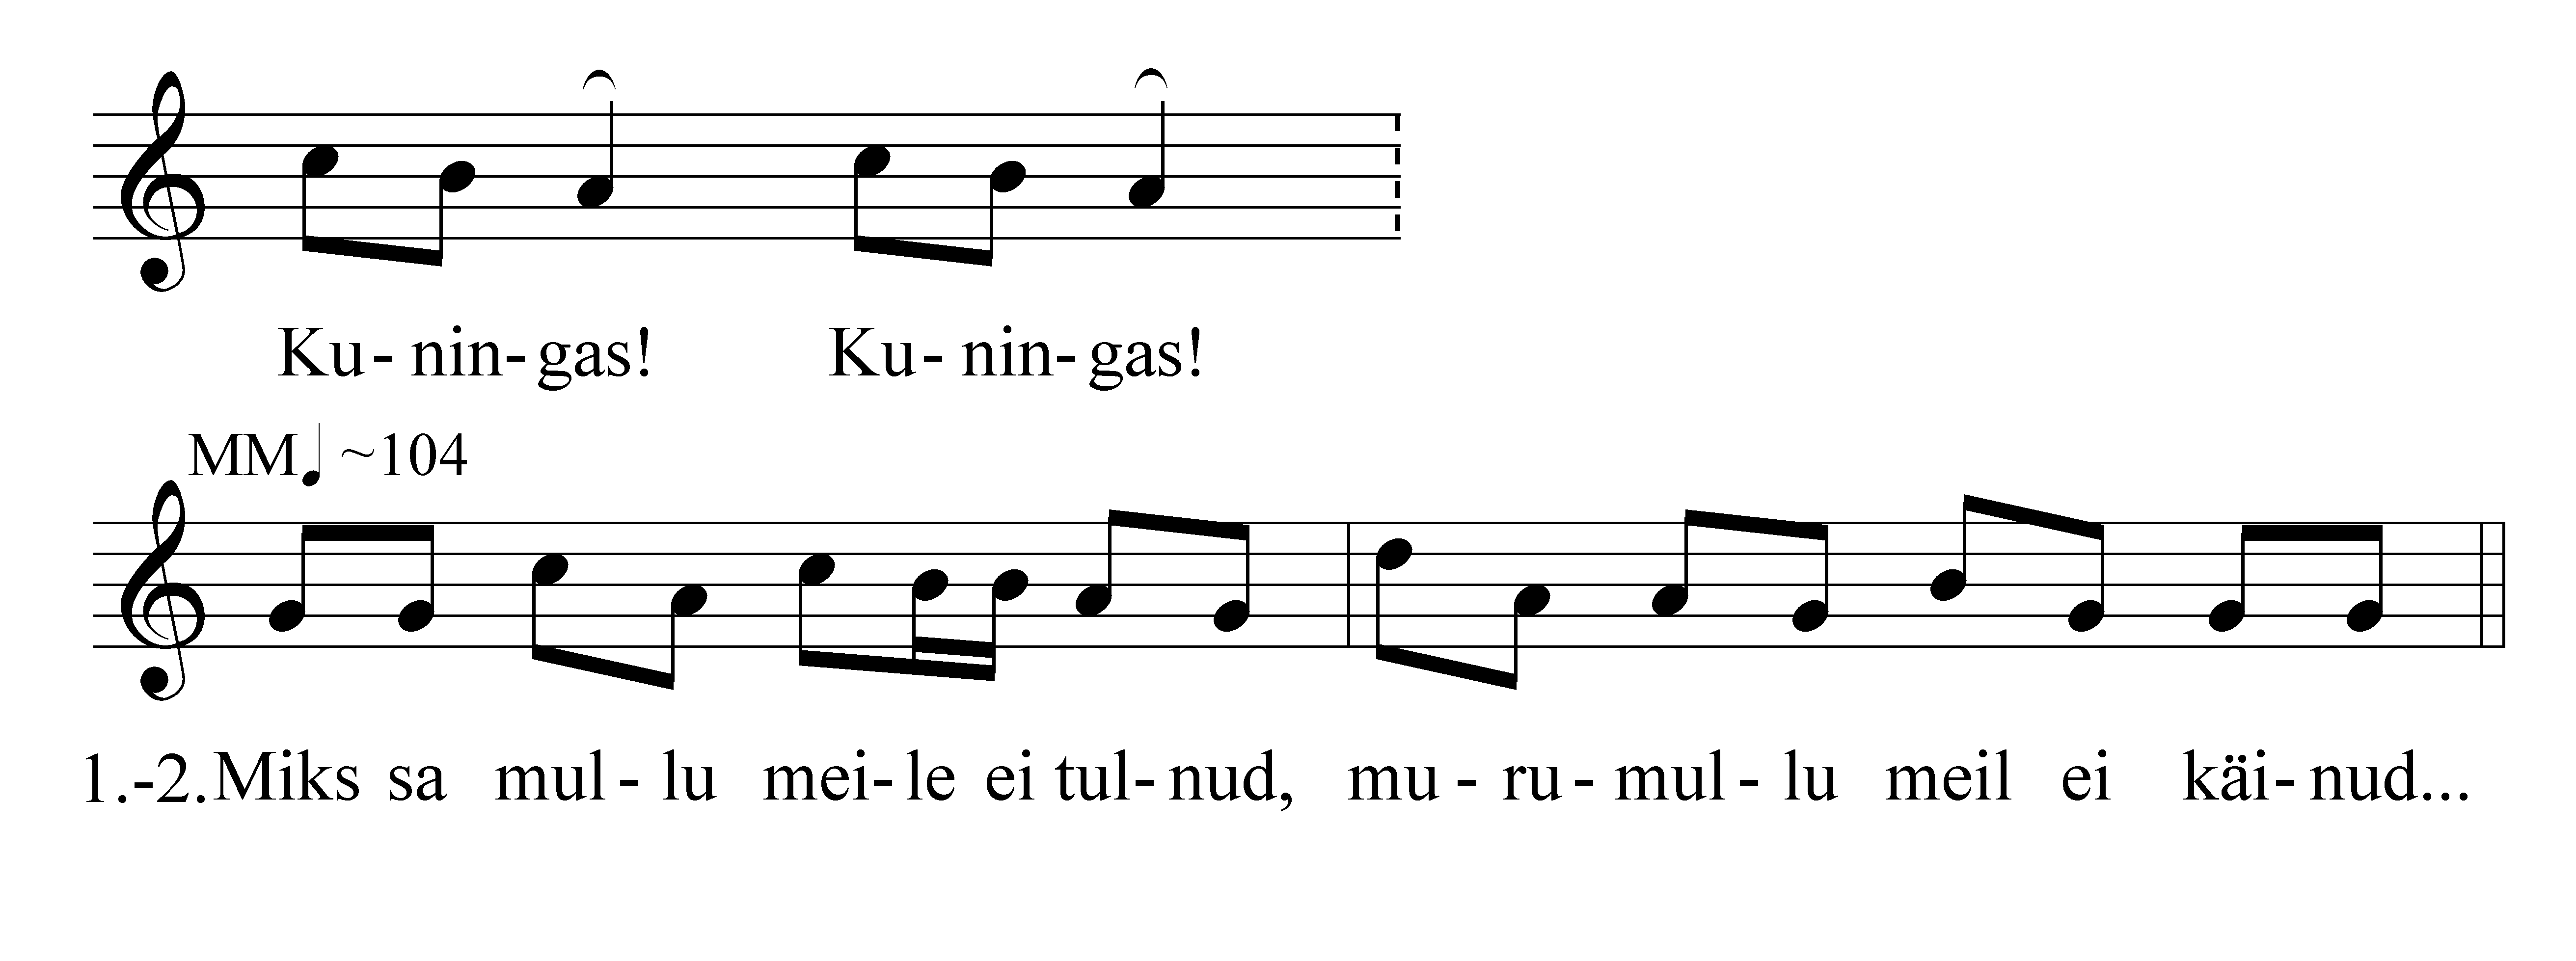
\includegraphics[width=300pt]{figures/094.png}
\caption{music notation of ``The King Game" as performed by Liisa Kümmel}
\label{The King Game}
\end{center}
\end{figure}

%\section{The Runic Song Tradition} 
%
%
%A given {\it regilaul} verse line contains eight beats, generally evenly divided into a single measure so that each of the eight syllables corresponds with one eighth note. The ictus position of a song's line is thus determinable by counting every other beat as ictus, starting with the first.
%
%The first song festival in Estonia held in \cite{ruutelTRADITIONALMUSICESTONIA2004}. 
%
%
%One runic invariant is that the tonal center is placed on ``the both syntactically stable 
%
%
%dominating pitch value of the most stable syntactical positions of a given melody's typological group
%
%
%the syllable-note is the basic unit of the melody-line. Thus syllables take up the space of the note in their position of the melody as prescribed. 

%Estonian, Finnish, Karelian, Ingrian runic songs
%
%whether it be Finnish, Estonian, Karelian, Votic, Ingrian and to same extent even Livonian an Veps)
%
%
the singable song \cite{tormis1985}
%
%
% ancient epic tale shared by many members of the Finno-Ugric language family
% 

 
 
 \cite{tormis2007}






 
\section{Previous Studies with regilaul}



The intuitions of ethnomusicologists who study the runosong tradition is that the burden of upholding the temporal structure of the song is the result of symbiosis between the musical rhythm and the natural prosodic features of the lyrical text \citep{ross1990, tampere1934}, inspiring over a decade of research at the interface of metrical phonetics and computational musicology. 
%
% 
%Melodic accents coincide with the stressed syllables, the pitch resolves as the phrase resolves. Said to be a musical abstraction of the natural prosodic intonation of the 8 syllable (spoken) runoverse \cite{ruutelResultsComputerizedComparative1999}.



\begin{figure}[htb]
\begin{center}
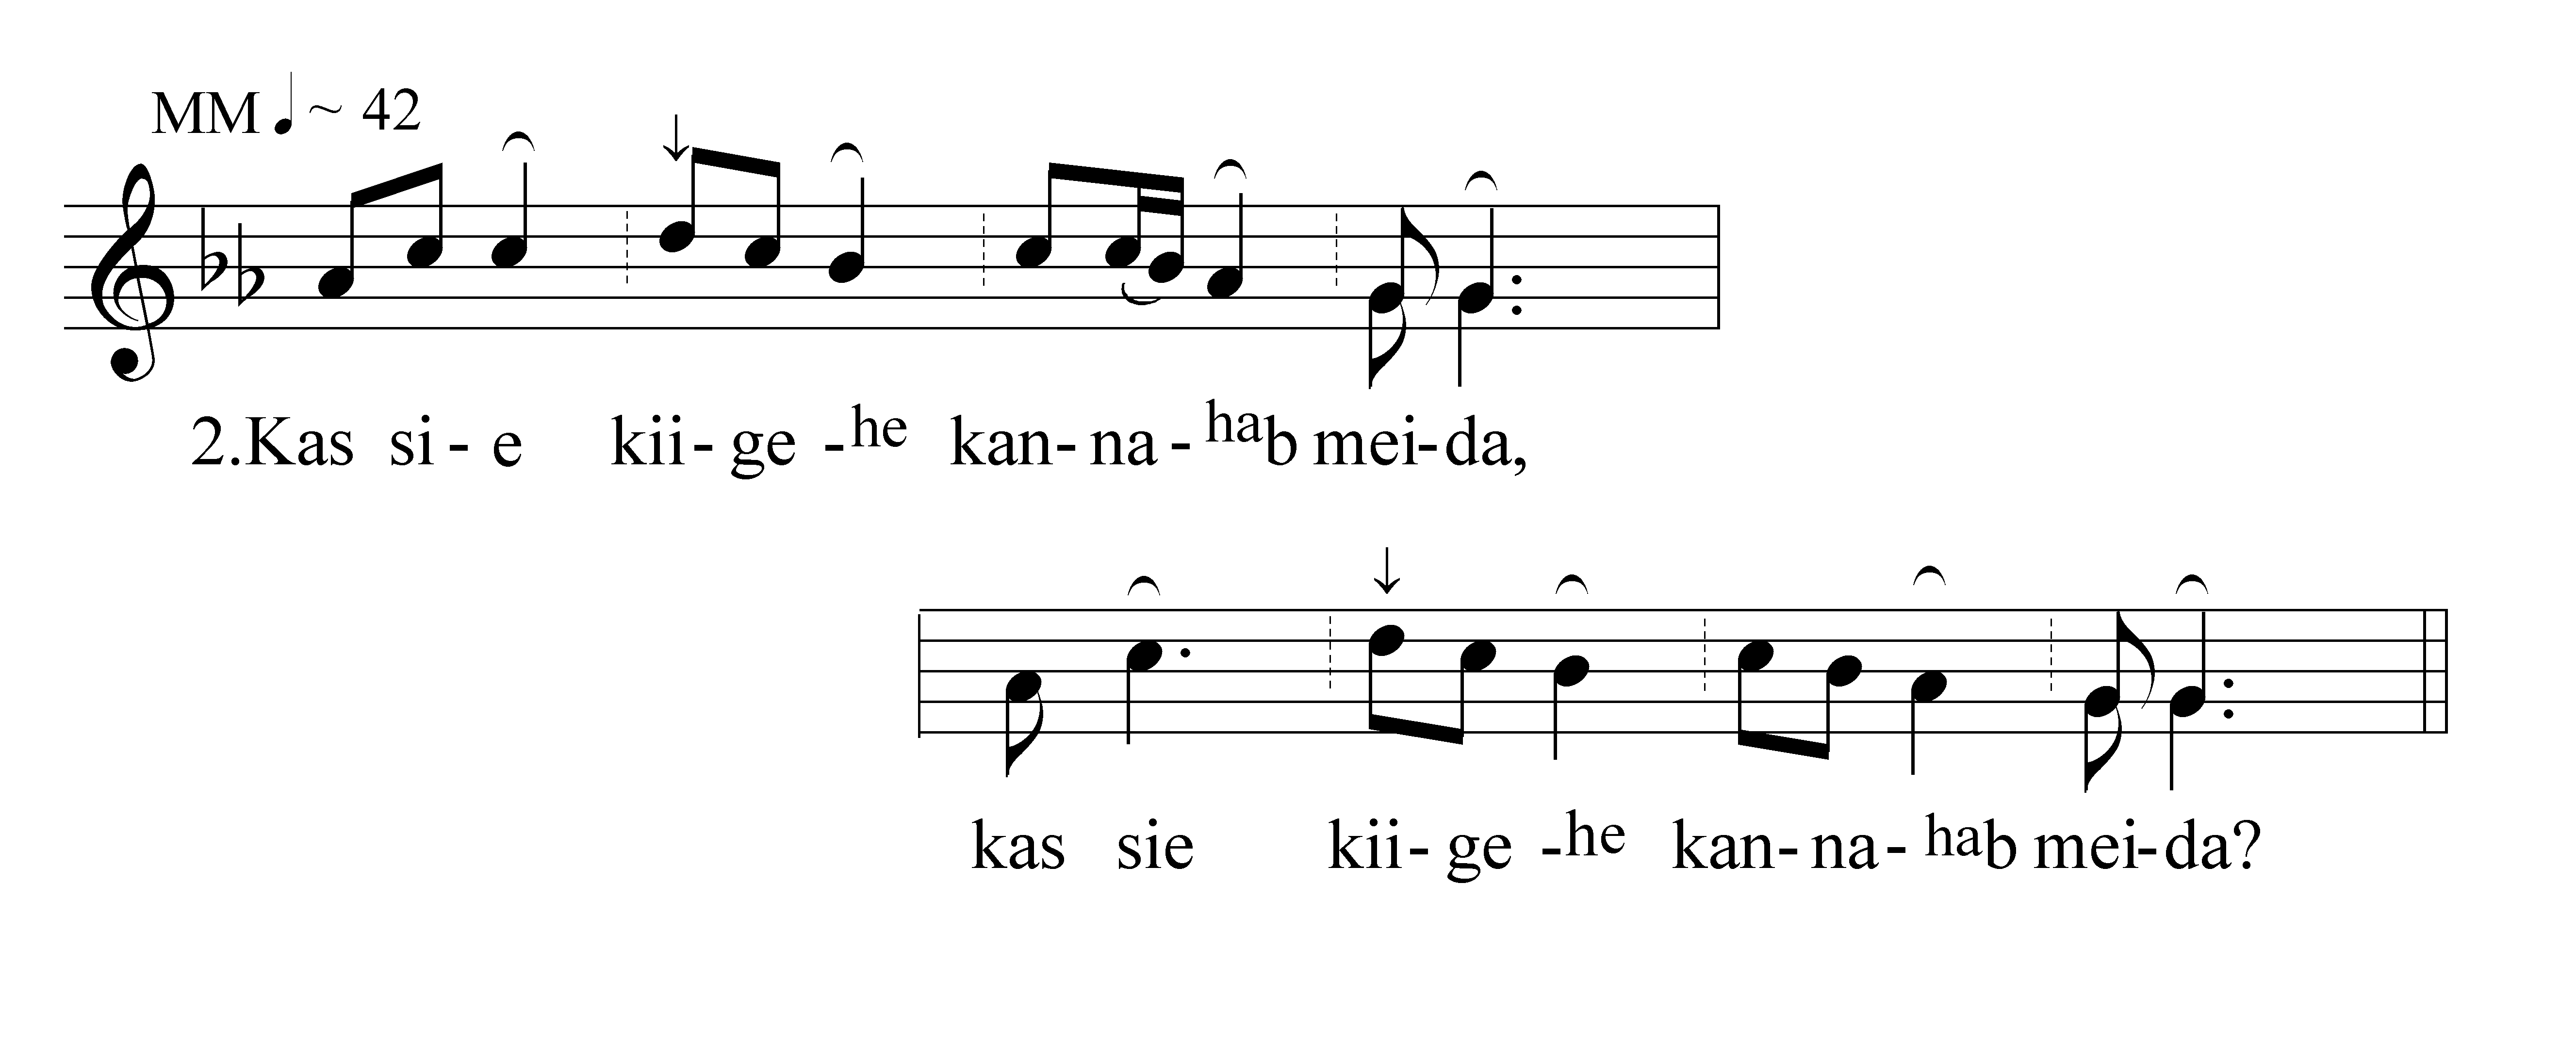
\includegraphics[width=300pt]{figures/022.png}
\caption{`Kiik tahab kindaid' \cite{}}
\label{022swing}
\end{center}
\end{figure}

Swinging songs are characterized by a swinging rhythm with alternating long and short notes, differing from the main body of {\it regilaul}'s iconic isochrony. 
Jaan Ross, a musicologist and native speaker of Estonian analyzed a 1936 recording of the swing song `Kiik tahab kindaid' \ref{022swing}, publishing results on syllable-note duration \cite{ross1989} and later the vowel quality of odd-numbered syllables \citep{ross90}. In the study on syllable-note durations, 

In the second, Ross measured formant frequencies f1 and f2, finding a reduced vowel space in song compared to measurements in spoken Estonian. However, upon examination of the song, it is clear that all the vowel space measurements are from syllable-notes in non-initial positions of Estonian words: that is, the sample of vowels taken from  the song were all unstressed, and compared to a mixed sample of spoken Estonian. Thus, the conclusion needs to be evaluated again with comparable samples. 

%
In 1992, Ilse Lehiste asked "Whether there is a correlation between poetic metre and the prosodic structure of a language.\citep{lehiste1992} by means of measuring the acoustic-phonetic realizations of so-called trochaic metrical poetic patterns across several languages including Estonian and Finnish. While these languages share in the more general Balto-Finnic tradition of {\it runosong} utlizing what is called the {\it Kalevala} meter, there were significant differences in the phonetic realizations of trochees in each language. 


In 1994, their collaboration begins. Ross and Lehiste published several papers examining the temporal dimensions of Estonian word prosody and metrical prominence in {\it regilaul} folksongs. In \citep{rossLehiste1994}, they conclude that duration differences ordinarily present at the word level (stressed-unstressed) are {\it ``lost"} to the temporal restrictions of the song. In another paper, syllable-notes are again measured, this time examining the role of syllabic quantity in the song. They likewise conclude that the duration of syllable-notes in {\it regilaul} match more closely with the metrical structure of the songs, that is, the durations of syllable-notes are best predicted by their beat position in the song: on the beat, syllables are longer, off the beat shorter. They extend this finding to conclude that the song "dominates" the metrical status of the words, claiming that the intelligibility of lyrics is enhanced more strongly by ``top-down" processes (i.e., semantic context). 

\citep{rossLehiste1996}. \\

%to paraphrase: Semantically relevant oppositions of word initial short-long and long-short disyllabic units in speech are not kept completely intact in folk songs. Short-long disyllables are treated in a different manner by the performer, depending on whether their initial syllable occurs at a rise or at a fall in a foot
\citep{rossLehiste1998} Analyzed and concluded that the {\it regilaul} lyrics are the result of an interaction between word and song prosodic hierarchies. This conclusion relied critically on measuring the durations of syllable-notes, where they found being on or off the beat was the better predictor for duration. \\


Finally, in %\citep{book_jril_2001} summarize their body of work until that point and extend their findings with fine-grained acoustic phonetic measurements of segment durations within syllable-notes. 

\section{The present study}

I do not dispute the findings that syllable-notes are best predicted by their position in the song. Instead, I argue that instead of an hierarchical interaction between language and music, what occurs is more akin to entrainment. Specifically, bidirectional entrainment of two oscillators. 

The syllable-notes, fit into the temporal structure of the music, still have possible acoustic-phonetic dimensions by which to indicate word boundaries (stressed-unstressed) and semantically-relevant quantity contrasts.  The durational differences of stress and quantity in spoken Estonian could be indicated either at another level of the prosodic hierarchy, i.e.,  the segment, or by enhancing another acoustic cue for prominence: i.e.,  vowel space dispersion. 


An EEG study of native Estonian speakers uncovered a perceptual asymmetry: shortening of constituents did not inducing MNN, but lengthening does \citep{eestiMNNasymmetry}. This suggests that stressed syllables, long in spoken Estonian, could be realized as shorter in a song without sounding ``off," but that lengthening of shorter elements would be less preferable. So long as syllable-notes maintain the relative durations in the song (i.e., heavy syllables are still longer than light ones), the metrical pattern of the musical phrase can be met. 

\subsection{Hypotheses}
Null hypothesis: on or off-beat position is best predictor for vowel duration of syllables in all categories: stressed, unstressed, short, long, and overlong. This would mean that the syllable nucleus is proportional to the total syllable duration, and that the duration contrast is indeed ``lost." 

H_{1}: duration contrasts for syllable quantity will be evident in the vowel duration, with vowel duration {\it decreasing} as syllable weight increases. Given the findings of \citep{rossLehiste2001}, isochronous syllable-notes would result in heavier syllables having shorter nuclei to accomodate for the coda and complex codas that distinguish the syllable weights from each other. 

H_{2}: stress/unstress contrasts will be evident in the nucleus in terms of hypo and hyper articulation. For this I measure both nucleus duration and vowel space dispersion. 

%\cite{rossStudyTimingEstonian1989,rossLostProsodicOppositions1994,rossTradeoffQuantityStress1996,sargDoesMelodicAccent2006, sargMelodicAccentEstonian2007,orasMusicalManifestationsTextual2011}

\chapter{Methods}
\index{Methods@\emph{Methods}}%


I first describe the source materials and the selection criteria for the sample corpus of {\it regilaul} folksongs. Following this, the annotation and measurement procedure is detailed. Then the procedure for assembling the corpus of songs and their text annotations is covered before proceeding to the inclusion criteria for vowel duration and dispersion measurements.


\section{Design of the Present Study}

autosegmental and segmental tiers

\subsection{Long Vowels and Diphthongs}
CV vs segmental dichotomy of CV phonology, as reflected in the suprasegmental aspects of vowels. 

An estonian word game supports the notion of many-to-one phonemes for long vowels, but a one-to-one status for diphthongs.



\begin{exe}

\ex  long vowels (Q1,Q2, Q3 contrast) 
	\begin{itemize} 
	\item sada `hundred' $\rightarrow$ sapida 
	\item  saada `send' (2nd sg. imp.) $\rightarrow$ sapiida (*sapiada)(*saapida)
	\item saada `get' , {\it -da} infinitive $\rightarrow$ sapii:da (*sapiada)(*saapida)
	\end{itemize}
\ex 	 diphthongs \\
laulus `in the song' (iness.sg) $\rightarrow$ lapiulus (*laupilus)
\end{exe}

In both cases, `pi' carries the prosodic characteristics of the displaced syllable. the stress is moved from first syllable to 'pi,' and also the length. crucially, the diphthong is split at the segmental level, while the long vowels are not. 

long vowels are treated as monophonematic, whereas diphthongs are treated as biphonematic. 

\cite{lehiste85, vago85}

As previous studies found that the durational properties of quantity contrasts were not found at the level of the syllable or the foot, I investigate the fine-grained acoustic-phonetic properties of these contrasts at the segmental level within the syllable-note of the song. 


To investigate the acoustic manifestations of stressed and unstressed syllables in {\it regilaul}, syllable nuclei from disyllabic feet in Q1 and Q2 are compared, as Q3 never appears in unstressed positions. 

Q1	CV 		CVC
Q2 	CVV		CVVC 	CVCC

The syllables are further compared by position in the song according to the beat: 

To investigate the question of quantity opposition in {\it regilaul}, disyllabic feet in Q1, Q2, and Q3 are examined according to their relationship to the beat. 



\subsection{segmentation criteria}

no syllables in verse-final or musical phrase-final position
vowel onset:
if sonorant onset, when intensity within 2 dB of steady-state/medial position of the vowel and intensity slope approaching zero
or the intensity slope approaching zero (less than or equal to one) for more drastic transitions such as obstruents
vowel offset intensity: before slope exceeds one (less than or equal to one) in transition to occlusion

primarily syllables with onsets

adjacent vowels across word boundaries, a glottal stop if present in the acoustic signal, otherwise omitted

lateral approximants in syllable onset usually easier to determine boundary, coda position /l/ no boundary definable and thus analyzed as a diphthong
in the case of intersyllabic long /l/, however, as there is no way to determine the end of the coda /l/ and beginning of the onset /l/, are excluded

song 41 contained churchbells
cases wherein word boundaries unclear due to transcription of the lyrics/poetic license

nonsense words

epenthesized vowels (i.e., pandi mind paju raiumaie) having mind(e) \\
word-final vowel next to word-initial vowel/difficult or impossible to determine end of preceding and onset of next across word boundaries


vowel onset and offset boundaries were determined using chiefly pitch and intensity contours in addition to the three first formants.



onsets: \\

plosive: not include burst. three first formants visible. slope of pitch and intensity contours encroaching on the respective steady state, with a slope less than or equal to one. 

liquids: formant steady state, steady pitch and steady intensity. 

nasals: intensity at least half of level within following vowel, antiformants, steady f0. intensity reduces in vowels. 

fricatives: following the end of the visible noise in the spectrum, at the point where intensity and formant contours are both visible and steady. The /s/  have reliable pitch carats immediately preceding vowels. \ref{spitch}. 

codas: \\

plosives: preceding fall in f0 and intensity
allow for more variation in formants of codas, other cues more consistent.

nasals: drop in f0, intensity less than half of the way to the level within-vowel. 

liquids: before drop in intensity 
before formant divergence.

across syllable and word boundaries: \\

adjacent vowels, when possible, segmented by presence of glotallization pulses and categorical changes in pitch. \\

In all cases, if the aforementioned cues are unavailable or ambiguous, the token is elided for this analysis. \\

A total of 757 individual vowel nuclei met the criteria for inclusion in duration measurements. After excluding diphthongs, a subset of _ met the criteria for inclusion in vowel space measurements. 


\subsection{Vowel Duration}
Why vowels and not entire syllables? The reason for this is twofold. First, measuring only the syllable nuclei affords more accurate automation. Were we to measure entire syllables, we would be limited to those with sonorant onset consonants, or in a restricted set of environments where consonant onset would be definable. By measuring only the syllable nuclei, we can reliably include more of the available vowel instances. Second, using the sonorant portions of the syllables makes way for the use of onset detection algorithms, so a strong beat is defined by a consistent threshold for each song, relative to the strength of the other beats in the signal. \\
The previous regilaul studies found evidence of syllable-note isochrony. So, if we see Q2 and Q3 vowels increasing in duration, this would be evidence against those findings. If, however, the long and overlong vowels have less duration than the short ones, this is evidence supporting syllable-note isochrony. Due to the structure of heavy syllables, the vowels must shorten in order to accommodate the additional coda segments within the note. 


\subsection{Vowel Space Area and Dispersion}

As a second measure of prominence, we include vowel space area and dispersion. Studies in English have shown that stress can be thought of as localized hyperarticulation or clear speech. \cite{deJong} Vowel space area and dispersion are well documented acoustic correlates of clear speech in English \cite{bradlow}, and has also been confirmed in cross-linguistic studies with Croatian \cite{rajka} and others. \\

While it has not yet been documented as an acoustic correlate of stress in Estonian, I have reason to believe that it will be an available cue for a singer to use, especially in the context of a song. While duration may or may not be an available prominence cue at the word level, vowel space area and dispersion are prominence cues that would not conflict with the prosodic hierarchy of the song. 

often, resonators or filters of musical instruments are solid or fixed. This is not the case with the vocal instrument.



then so long as the word-level categories of quality are preserved, the 


\section{Materials}

\begin{figure}[htbp]
\centering
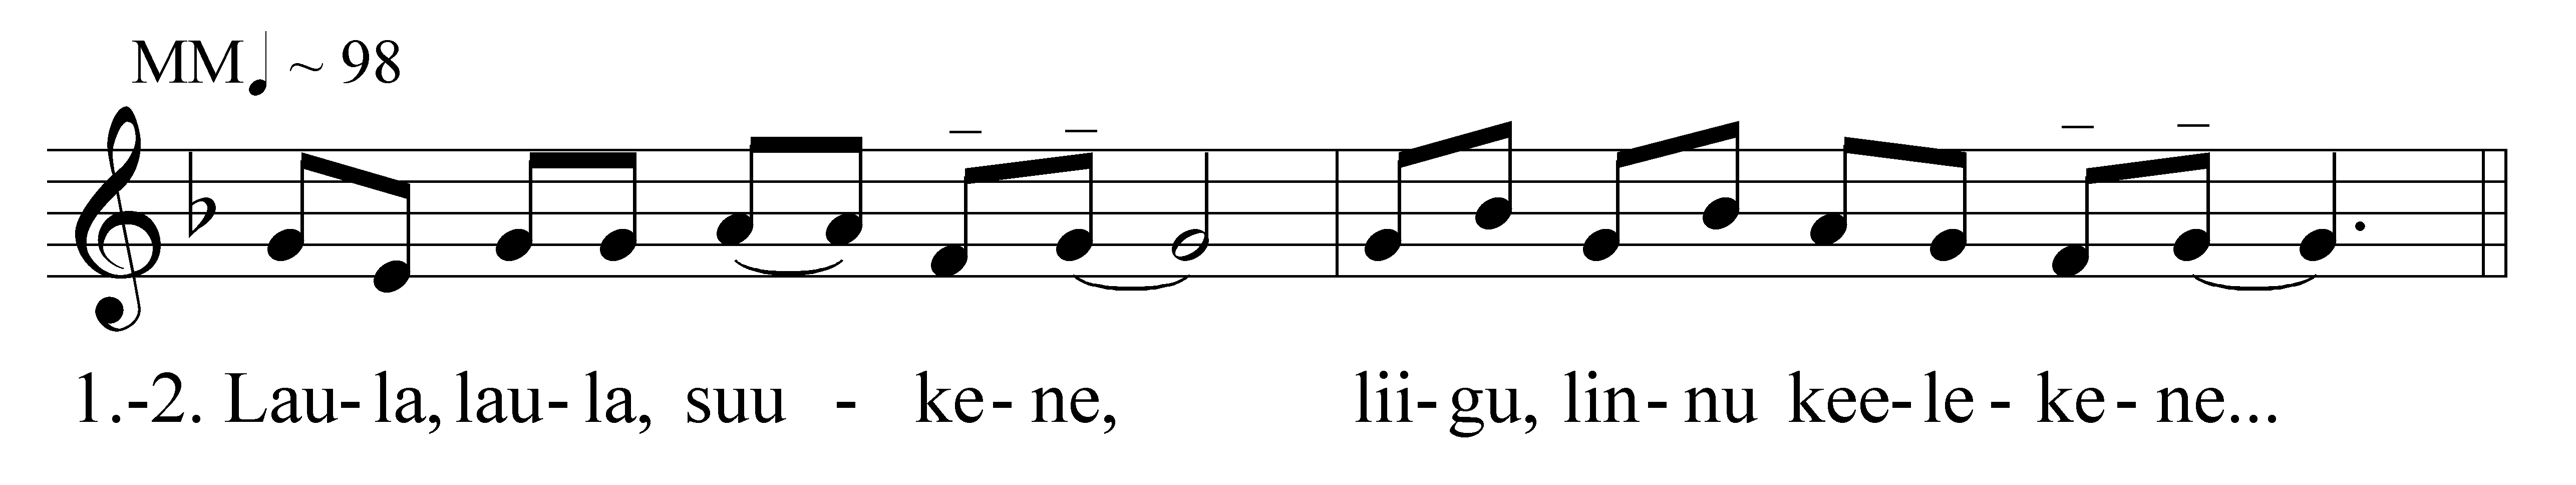
\includegraphics[width=300pt]{figures/055.png}
\caption{Laula! {\it Sing!}}
\label{default}
\end{figure}




The data for this study was sourced at the Estonian Folklore Archives (EFA). 
\citep{orasEstonianFolkloreArchives2022a}.



Until 1948, songs were collected on wax cylinders, then played on a phonograph and transcribed. shellac discs 1936-38, 746 recordings, 
analogue is the biggest collection in the archive, with over 80,000 individual recordings. Open-reel tape, cassette recordings since the 1970s. 
both wax and disc were re-recorded onto open-reel tape in 78-79.
Presently, the sound engineer Jaan Tamm has been working on preserving the earlier tape recordings in digital form for the EFA. WAV files are stored on CD-Rom at the EFA in Tartu, Estonia, while .mp3 and .ogg lossy formats are uploaded to the internet database. 
% collected by Herbert Tampere, Erna Tampere, and Ottilie Kõiva between 1912 and 1966 for the Estonian Folklore Archives in Tartu, Estonia. \\
%
% and   tunes
%the total number of song recordings is over 26,000. Of these, over 11,000 are from the beginning of the 20th century. Tampere did like 2,000 of them..
%
%%
%The need for writing the tunes live during fieldwork has reduced with the availability of analog and now digital audio recording equipment.




Songs for this paper were accessed via The Anthology of Estonian Traditional Music \citep{tampereAnthologyEstonianTraditional2016}. Originally published on four vinyl discs in 1970(\ref{vinyl1970}, the digital version showcases a robust sample of the massive collection of {\it regilaul} in Estonian Folklore Archives. In addition to audio, the  compilation includes  photographs, sheet music, and performer demographics of 98 {\it regilaul} songs and 17 instrumental tunes. 
These songs were compiled in part by Herbert Tampere, an early ethnomusicology field work organizer of the EFA, who along with Erna Tampere and Ottilie Kõiva collected these folk songs. Pictured in \ref{tampy} is a photograph taken of one of the very field trips to record songs studied in this paper. 

\begin{figure}[htb]
\centering

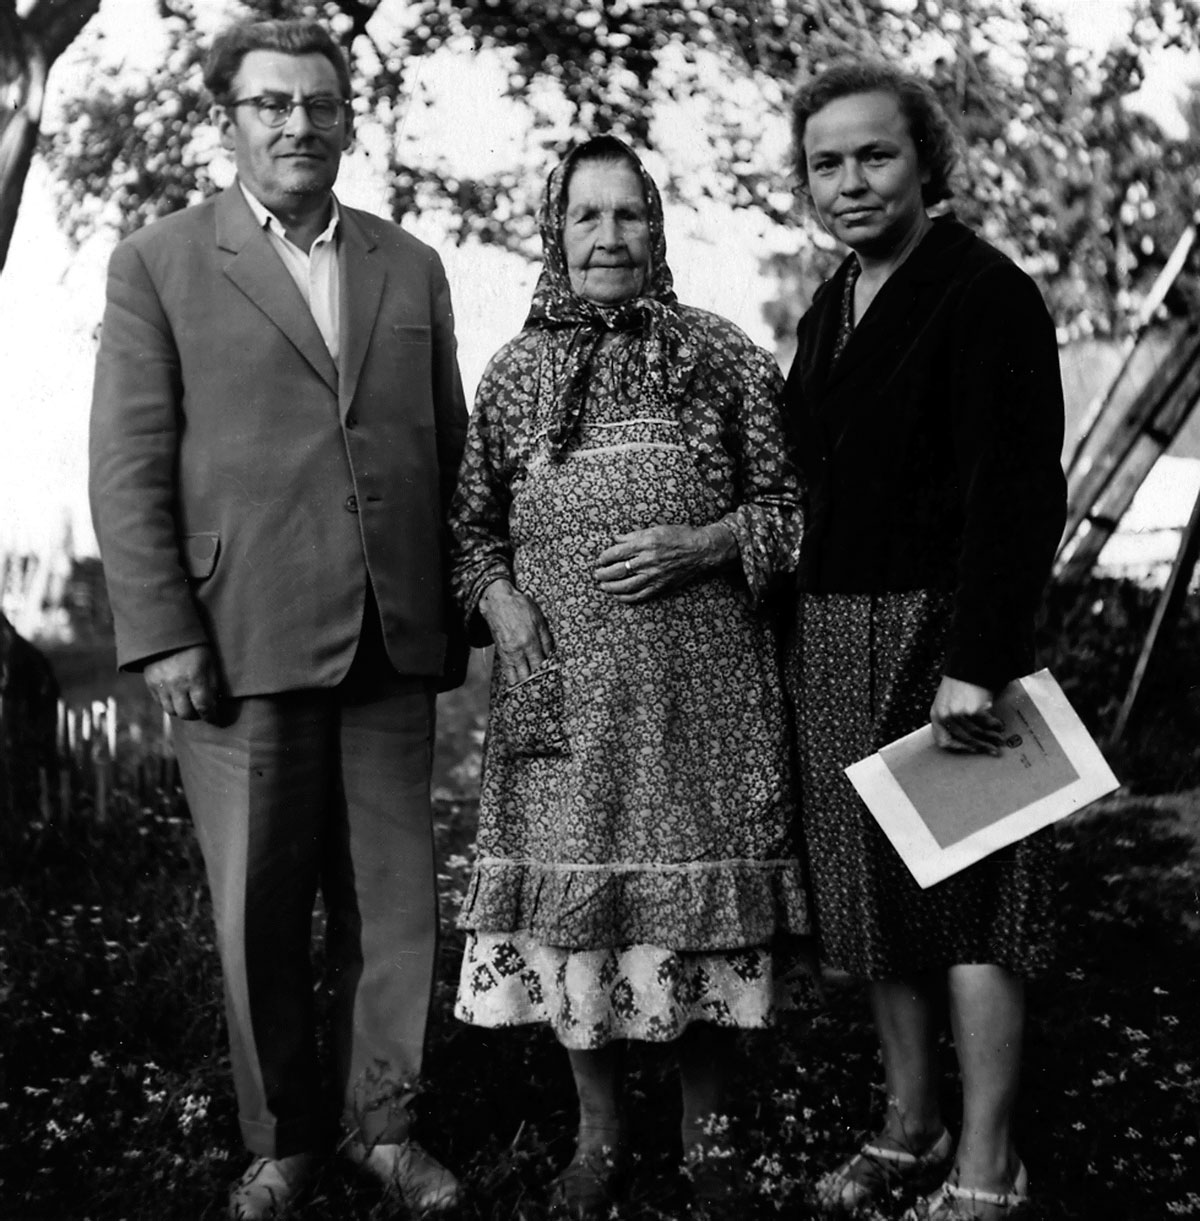
\includegraphics[width=200pt]{figures/Mf_07027_Tampered_Orik.jpg}
\caption{Herbert Tampere on a field trip}
\label{tampy}
\end{figure}


While the ultimate goal is to continue annotation of the entire available corpus of {\it regilaul}, for the initial analysis I chose a sample of songs all belonging to the same regional dialect and recording method. Once several regions were identified as possible candidates, a native Estonian speaker was consulted on the final selection. The nine songs analyzed in this study were all recorded in Parnümaa county from 1961-1966 by Herbert and Erna Tampere. 
% The first criteria is due to the lossy nature of some of the older files available on the site: the online versions are all compressed lossy, so the analog audio originally recorded on tape and then digitized have a higher resolution, even compressed, than songs that have been copied from wax cylinders or shellac discs onto open-reel tape and then digitizing. 


\section{Annotating the Song Audio }



 Each song's lyrics are copied from the site and saved as .txt files in Estonian orthography, each line of the file corresponding to one melody line.  
Audio files of the selected songs are downloaded from the archive in .ogg format, which is the highest resolution of the two lossy\footnote{define lossy} formats available from the digital anthology. Each song is then imported into a Logic Pro X \citep{b131156} session for beat detection, tempo mapping, and trimming. 
To make the tempo map, the session must be set to {\it flex tempo}. From here a beat onset detection algorithm \citep{robertsonBKeeperBeattrackerLive2007} is  given the transcribed bpm and time signature from the archived song data and run on the imported audio file. The result is an annotation of intervals in time, and the bpm for each measure is annotated according to the performance of the song.
The tempo map allows us to document when {\it exactly} in time the particular singer performed a given note, the duration of the sung note, and the acoustic threshold by which the note is defined as ``strong" relative to surrounding notes. The process is informed by the transcribed bpm and time signature included in the anthology. This is beneficial to my purposes in two ways: by accounting for the natural tempo variation in live performance, and by using a consistent metric to determine beat strength acoustically rather than just perceptually.

 From here, a MIDI track is programmed to create a metronome that is the length of a single syllable-note in the song. In most of these, a 4/4 measure contains eight eighth notes, so the metronome track contains four eighth notes indicating the ``ictus" beats. In flex tempo mode, the MIDI track adjusts note and measure length to match the fluctuations in tempo as documented in the map for the song. The metronome and the song audio file are trimmed to match exactly, and the metronome is converted into a textgrid in PRAAT\citep{boersnaPraatDoingPhonetics2022}, where the annotation process continues. 

 


The orthographic text phrases of the song lyrics are then inserted into each phrase interval with a script, and then eSpeak forced aligner for Estonian \citep{duddingtonESpeakSpeechSynthesizer1995} is run on each phrase to the word and phonemic level. Because this forced aligner is trained on spoken, not sung Estonian, the aligner sometimes tries to align words into the signal before they are uttered. In these cases, the word level tier is manually realigned so that it contains all and only the transcribed word, and then the forced aligner is re-run on this word to the segmental level. In the case of a vowel interval containing an obvious silent portion or occlusion, the boundary is manually adjusted to only include sonorant portions of the signal. 
% \begin{figure}[ht]
%\begin{center}
%			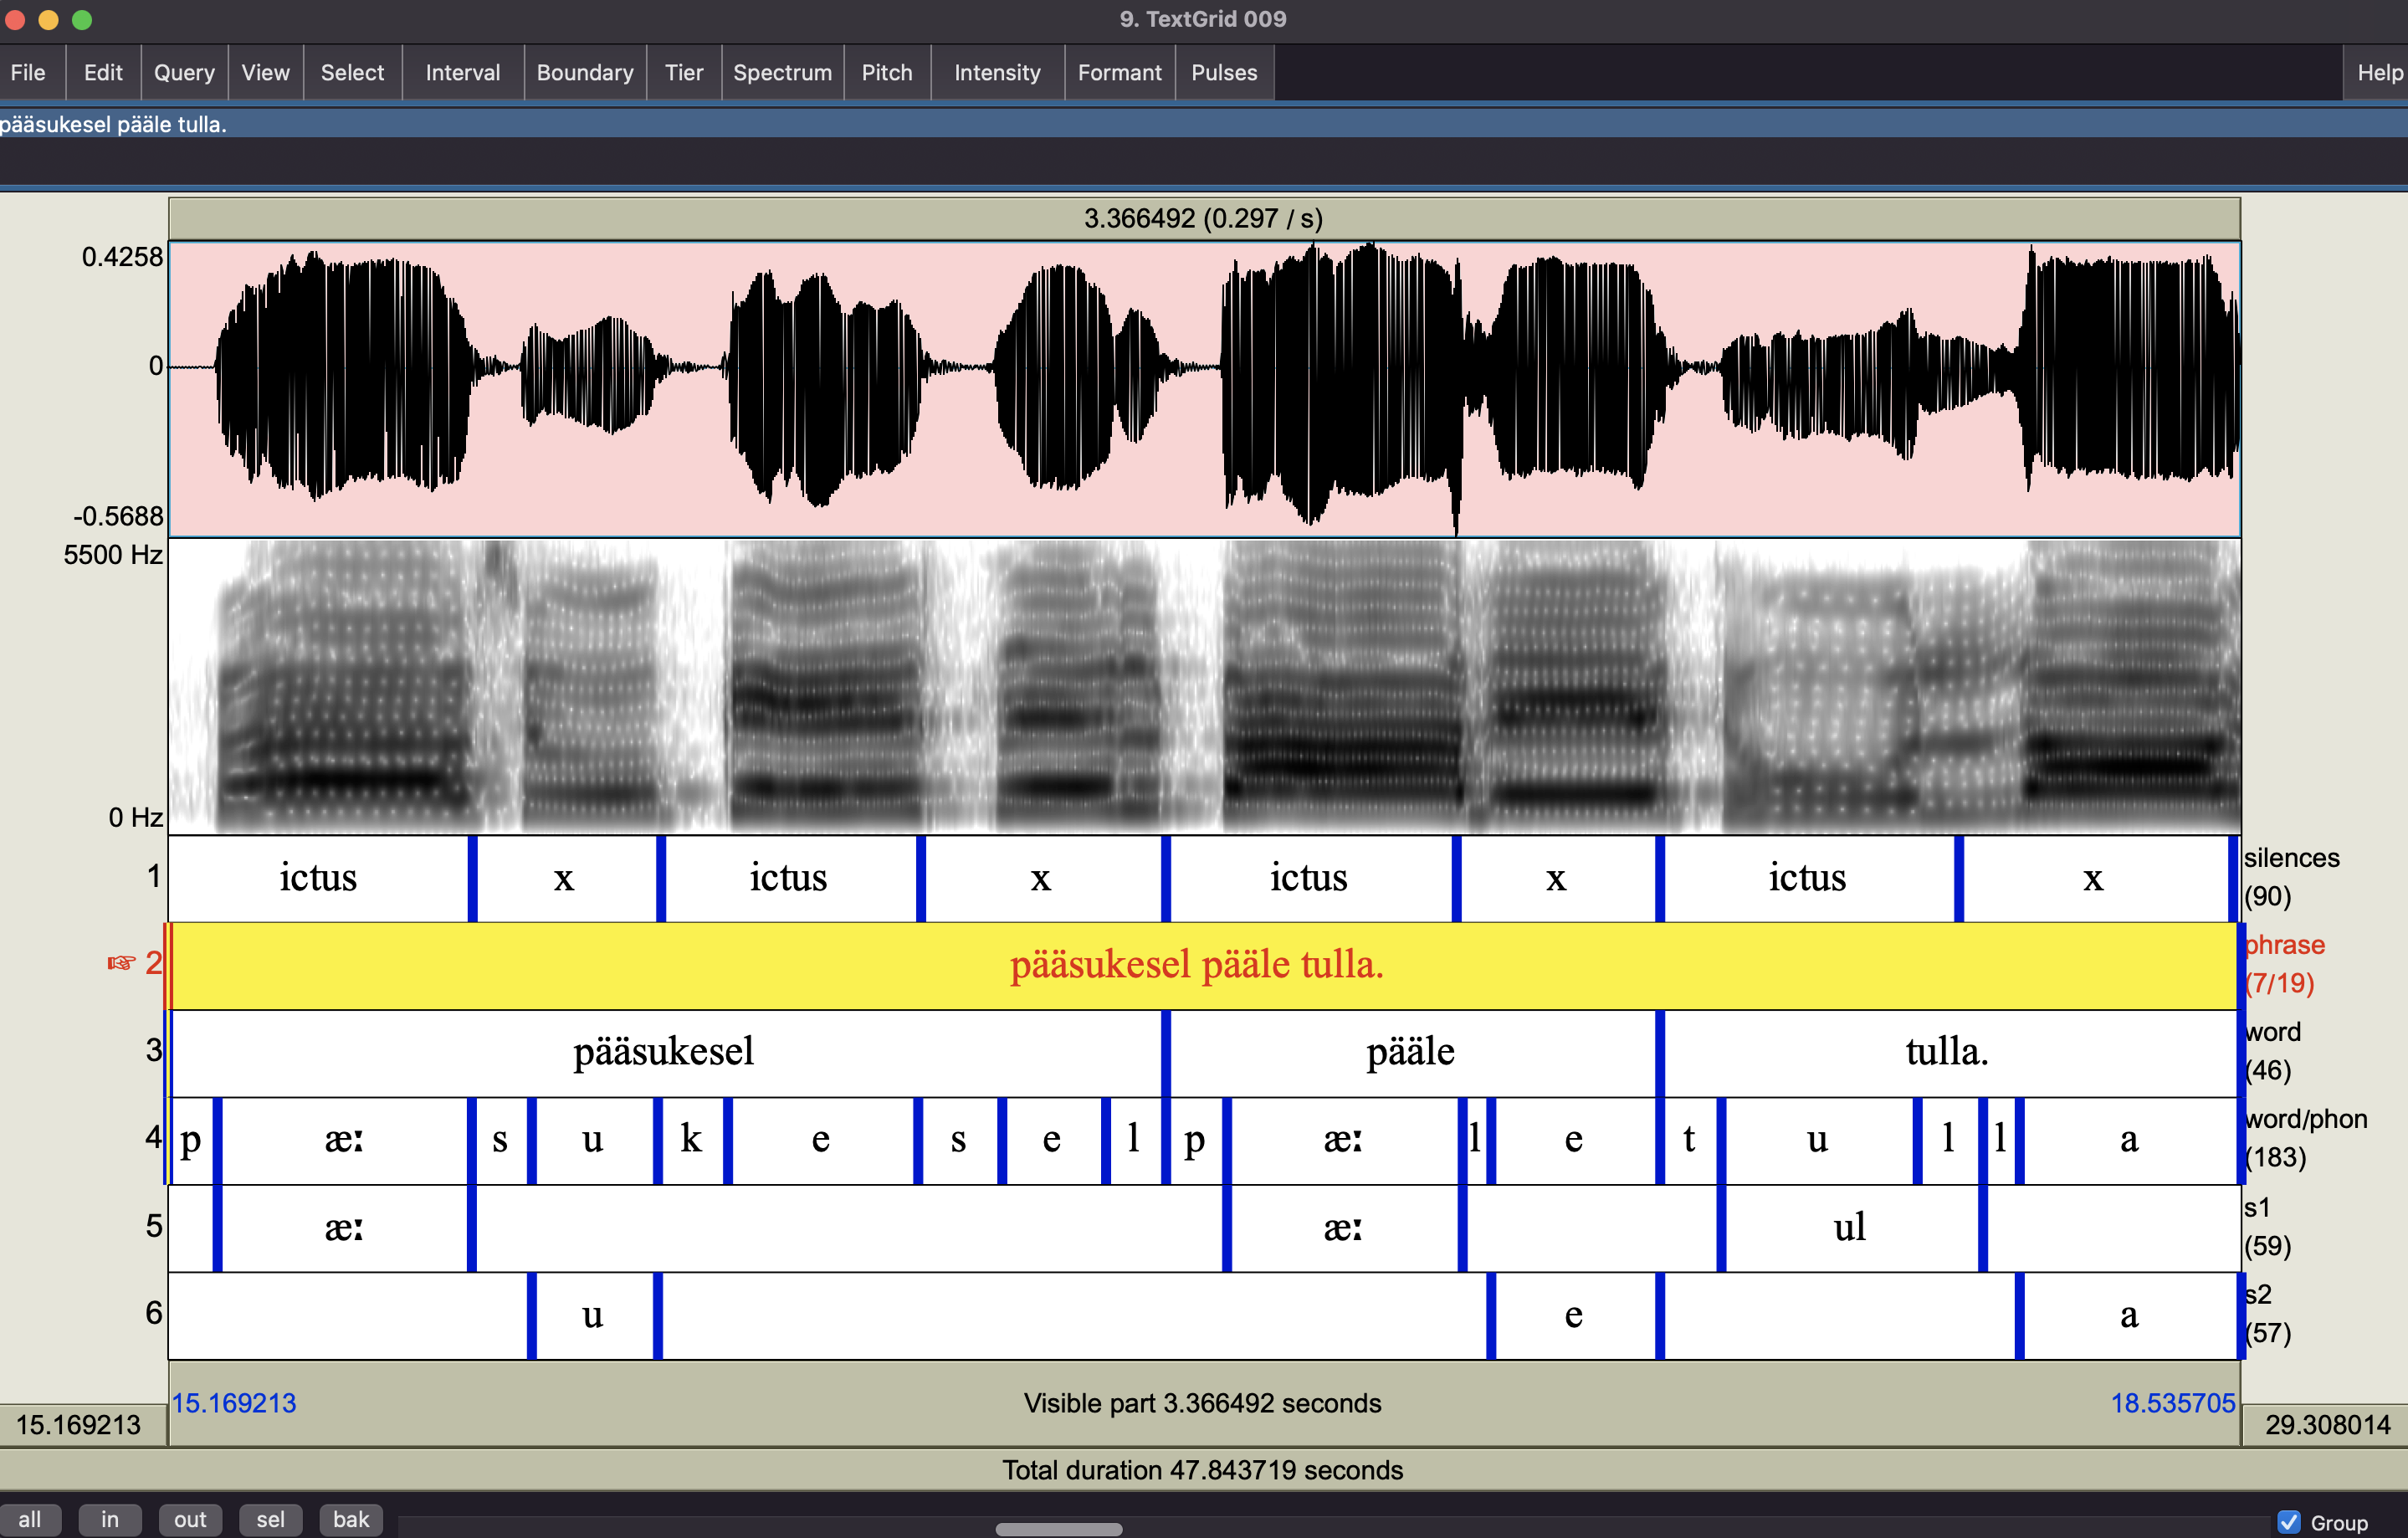
\includegraphics[width=300pt]{figures/phrase_grid.png}
%			\caption{single phrase annotation}
%\label{phrase}
%\end{center}
%\end{figure}
%\begin{figure}[hb]
%		\begin{center}
%			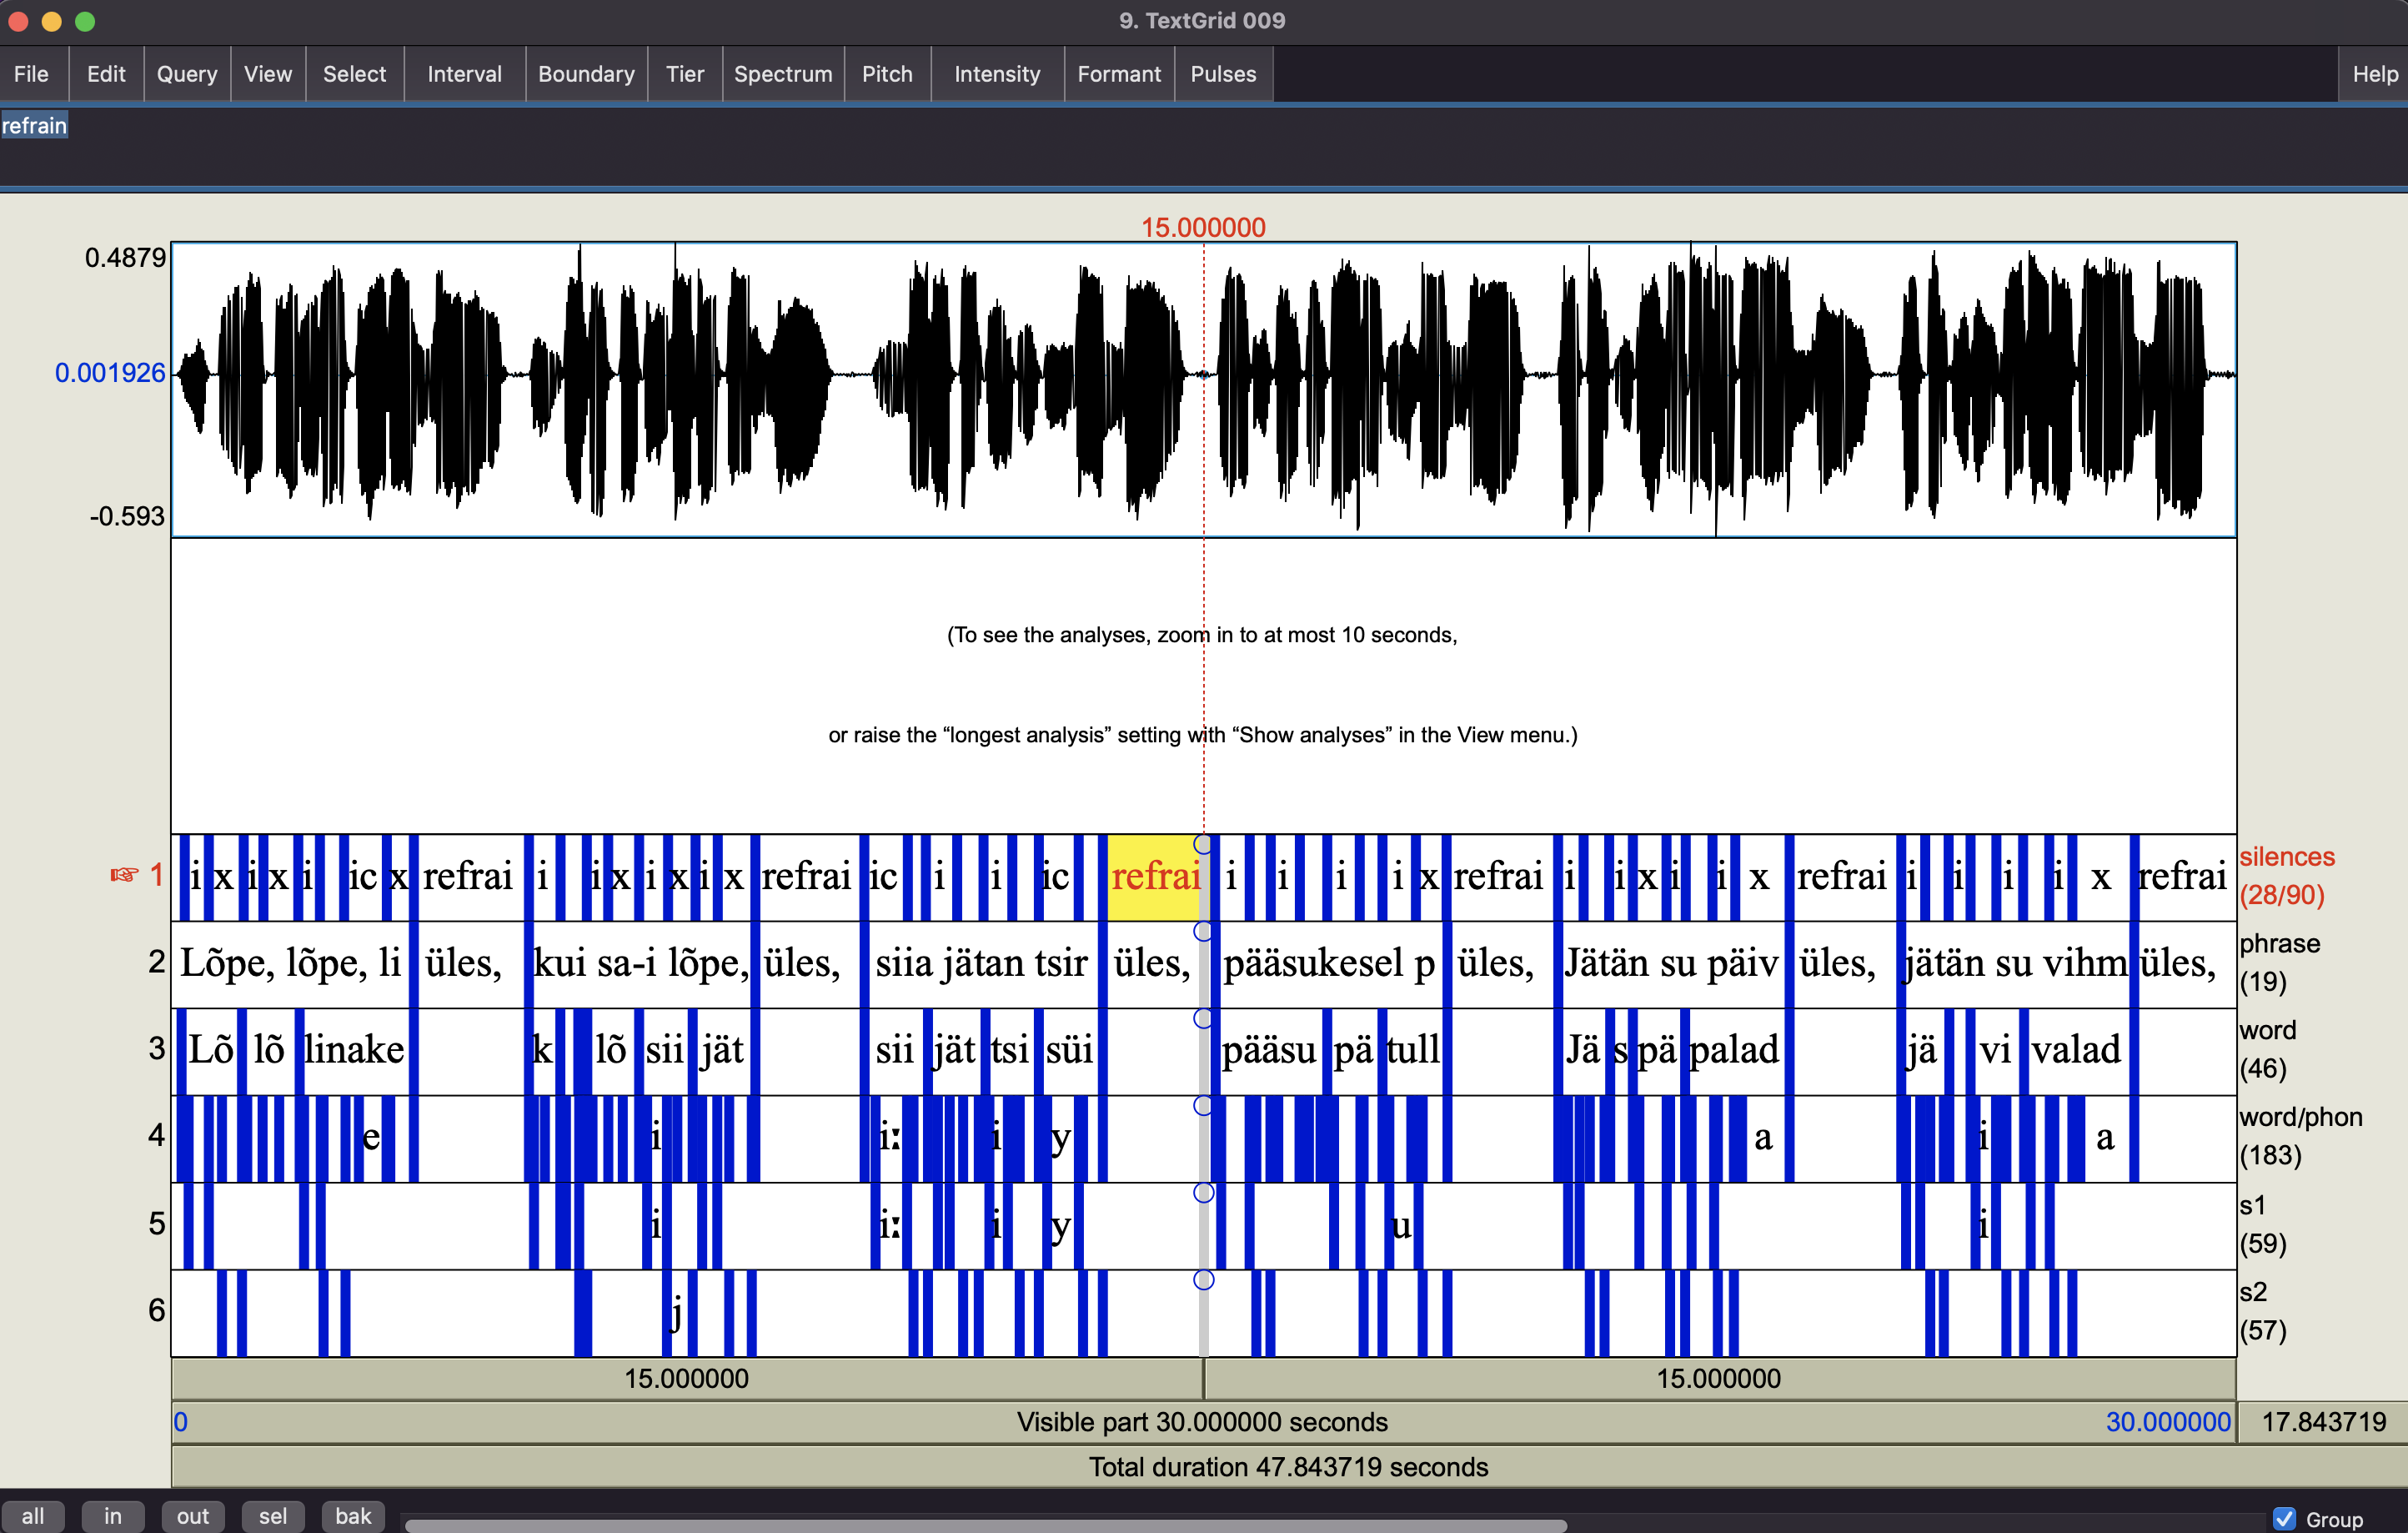
\includegraphics[width=300pt]{figures/big_grid.png}
%			
%			\caption{whole song annotation}
%			\label{songwhole}
%		\end{center}
%\end{figure}
%	
%	 In \ref{phrase} is a completed annotation of a single phrase from a song, and in \ref{songwhole} is an entire song file's interval annotation.

At this point, the audio recording of each song has tiers annotated for tempo and strong beat, verse line phrases, two interval tiers force-aligned to word and phoneme levels, and a separate tier with intervals of the individual vowel segments of interest copied from the phoneme tier.
\section{Assembling the corpus and annotations}
The last step in preprocessing is to integrate the annotation of the song audio with the lexical content of the song. This study accomplishes the task using an open-source natural language toolkit in python called estinltk \url{https://github.com/estnltk} \citep{laur-EtAl:2020:LREC}. Among other things, the toolkit has a robust dictionary of Estonian grammar, including phonetic transcription of syllables with quantity and stress data. 


Thus the data structure of this corpus offers two independent metrics of rhythmic prominence in these songs. From the audio recording and the beat detection, we have an annotation of strong beats based on replicable acoustic measurements, and from the dictionary in the natural language toolkit, we have native speaker intuitions about the lexical weight and prominence in the words of the text. While the stress system is generally predictable, the syllable quantity is not always apparent from the orthography, and not always detectible by a non-native listener. Linguistic descriptions of the Estonian language date back as early as the seventeenth century, but the ternary quantity contrast was not documented until native Estonian linguists contributed their intuitions. The non-native linguists had only described lexical stress \citep{sargEarlyHistoryEstonian2005a}. \\

Using onset detection algorithms such as these \citep{robertsonBKeeperBeattrackerLive2007} in phonetics research, especially in the interdisciplinary field of linguistics and musicology, will be particularly beneficial to answering questions about rhythm: finding a way to bring our intuitions and impressions about ``the beat" together with the acoustic phenomenon. By automating the annotation and measurement process using open source tools, the author hopes to share these machines with those who have similar research interests, and also to invite contributors to the data of this corpus of text data time-aligned to queryable audio signal data. 

\section{Study Design}
\subsection{Questions and Hypotheses}

\subsection{Inclusion Criteria for Vowel Measurements}

Once the annotations are complete, the corresponding text files are aggregated and, the corresponding measurements from PRAAT are concatenated via python using the parselmouth library python interface to PRAAT \citep{parselmouth, van1995python}. 
 I extracted vowel intervals which met the following inclusion criteria. For this study, we are interested in the durations of vowels in initial and pen-initial syllable-notes that are transcribed as isochronous in the melodic transcription. 

\subsection{Statistical Analysis} 
Linear mixed-effects model using lme4 in R \cite{rlme4}. 

For stress and ictus, only q1 and q2 syllables (Q3 never unstressed). \\
for quantity and ictus, only word-level stressed syllables



Design-based formula
Hierarchical Linear Model with group-specific terms

\cite{goodrichRstanarmBayesianApplied2020,brillemanJointLongitudinalTimetoevent2018}

\chapter{Results}
\index{Results@\emph{Results}}%

\section{Quantity Oppositions in Ictus position}


Ternary quantity contrast is only in primary stressed syllables. To analyze vowel duration measurements in all three quantities, a subset of only primary stressed syllables is taken from the dataset. 
At the song level, the kalevala meter avoids short stressed syllables (Q1) in ictus position, preferring Q2 or Q3 (long and overlong) syllables to fall on the beat. In off-ictus postion, short stressed (Q1) syllables are preferred while Q3 avoided.


\begin{figure}[htb]
\centering
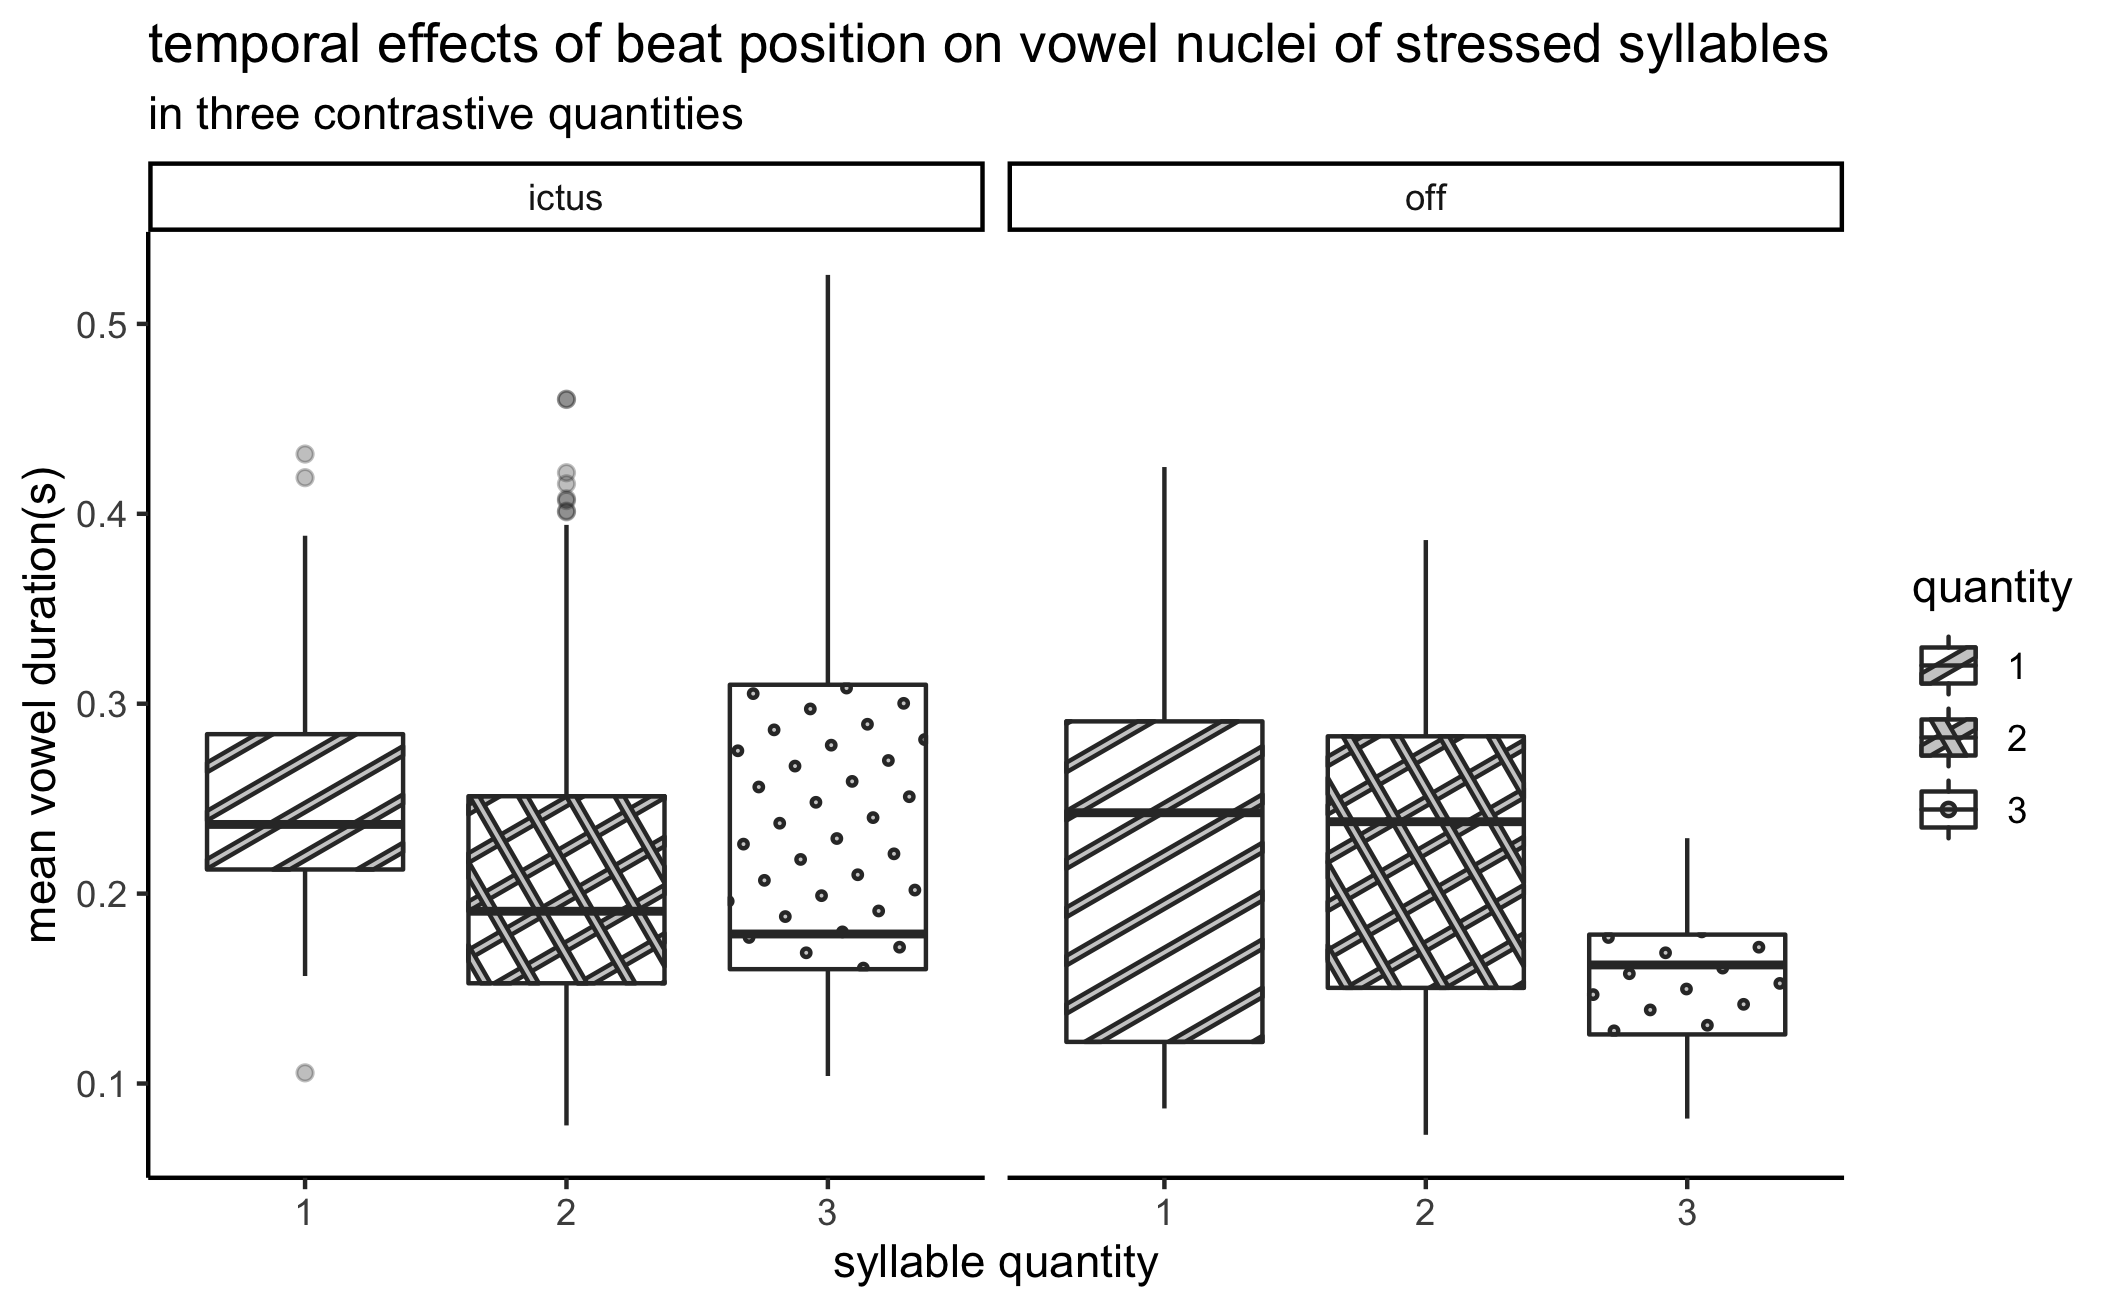
\includegraphics[width =\textwidth]{/Users/sarah/Git/regilaul_project/manuscript/results/q_dur.png}
\caption{density plot of vowel durations in three syllable quantities}
\label{qdur}

\end{figure}
%\begin{wrapfigure}{l}{\textwidth}
%\centering
%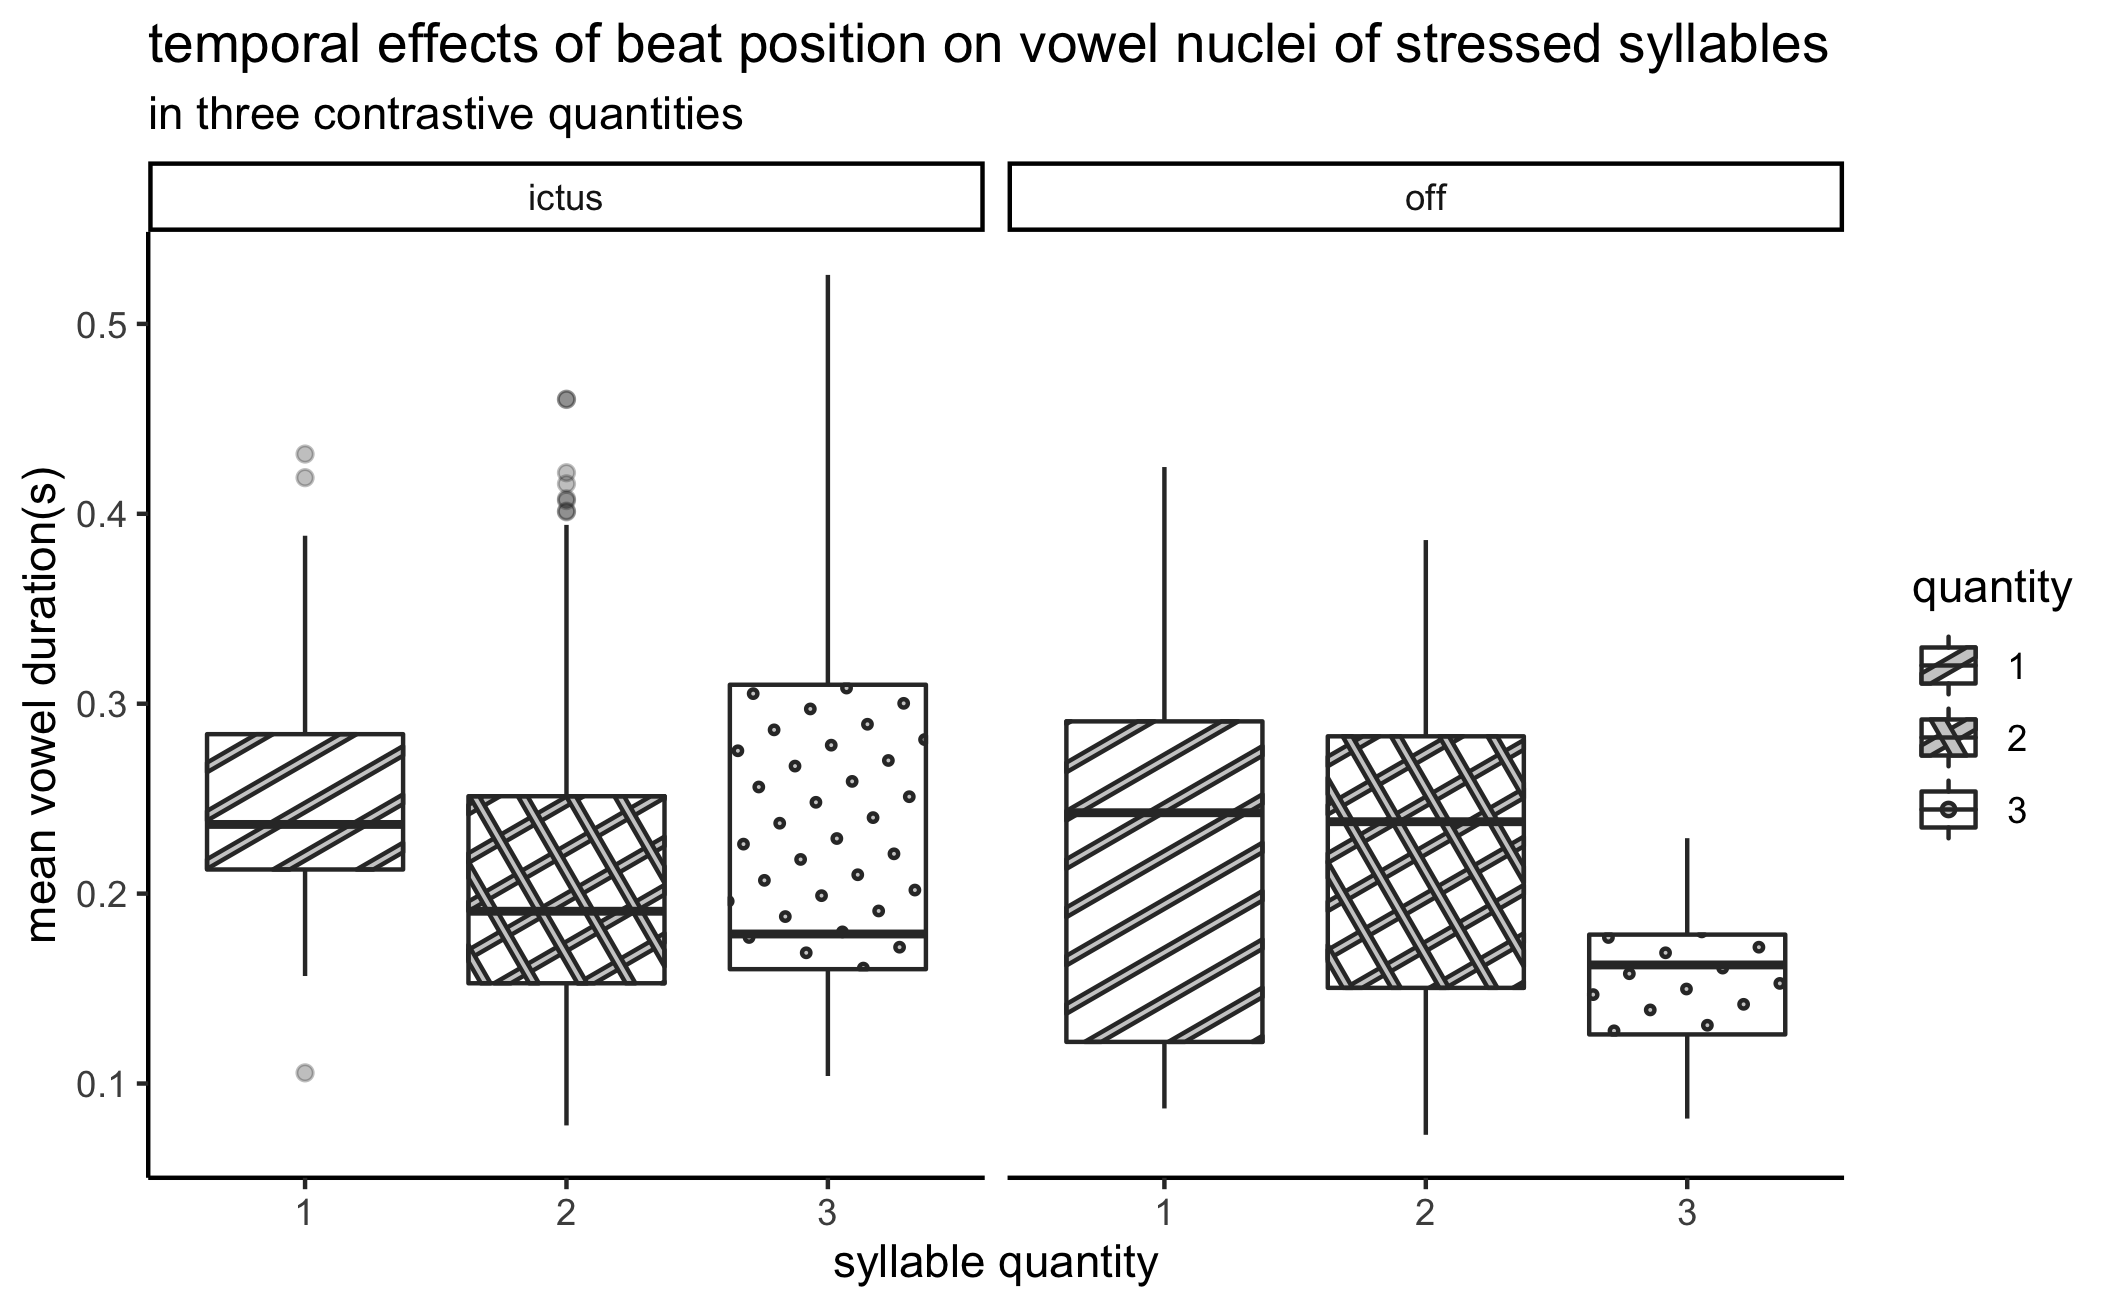
\includegraphics[width =\textwidth]{/Users/sarah/Git/regilaul_project/manuscript/results/q_dur.png}
%\caption{density plot of vowel durations in three syllable quantities}
%\label{qdur}
%
%\end{wrapfigure}


\ref{qdur} shows the vowel durations of all three syllable quantities, grouped by ictus and off-ictus positions in the song. In ictus position, median vowel duration descends as quantity increases, with the greatest difference between Q1 and Q2. Off the beat, a similar descending pattern is evident: however, in this case the largest difference is between Q2 and Q3 syllables. 
 The intercept is set at ictus position, Q1. Findings are significant results for Q2(p<0.001), Q3, and off-ictus positions (p< 0.05). Comparison with null model was statistically significant (p<0.001). For full model output see \ref{qdurfixed} and \ref{qdurrandoms} in Appendix A. In context of earlier findings that the quantity contrast was ``lost" at the syllable level, the decrease in vowel duration as syllable weight increases supports the notion that the contrast is preserved at the segmental level. That is, rather than the full syllable lengthening in duration, the song-level isochrony of syllable-notes results in vowel nuclei shortening to accommodate codas in Q2, and further for geminates and complex codas in Q3. 
 
 
A null model constructed containing only random effects was compared to the design model by two-way ANOVA. Results are significant for the design model (p < 0.001***), and so I reject the null hypothesis. 

These data and analysis support both syllable quantity and ictus as predictors for vowel duration. 



%\begin{equation}
%$$lmer(duration ~ quantity + ictus + quantity * ictus + (1 | song) + (1 | word) + (1 | performer))$$ \\
%
%$$lmer(duration ~ (1 | song) + (1 | word) + (1 | performer))$$
%
%
%
%\end{equation}
\section{stress and unstress}


\subsection{duration}

\begin{figure}[htbp]
\centering
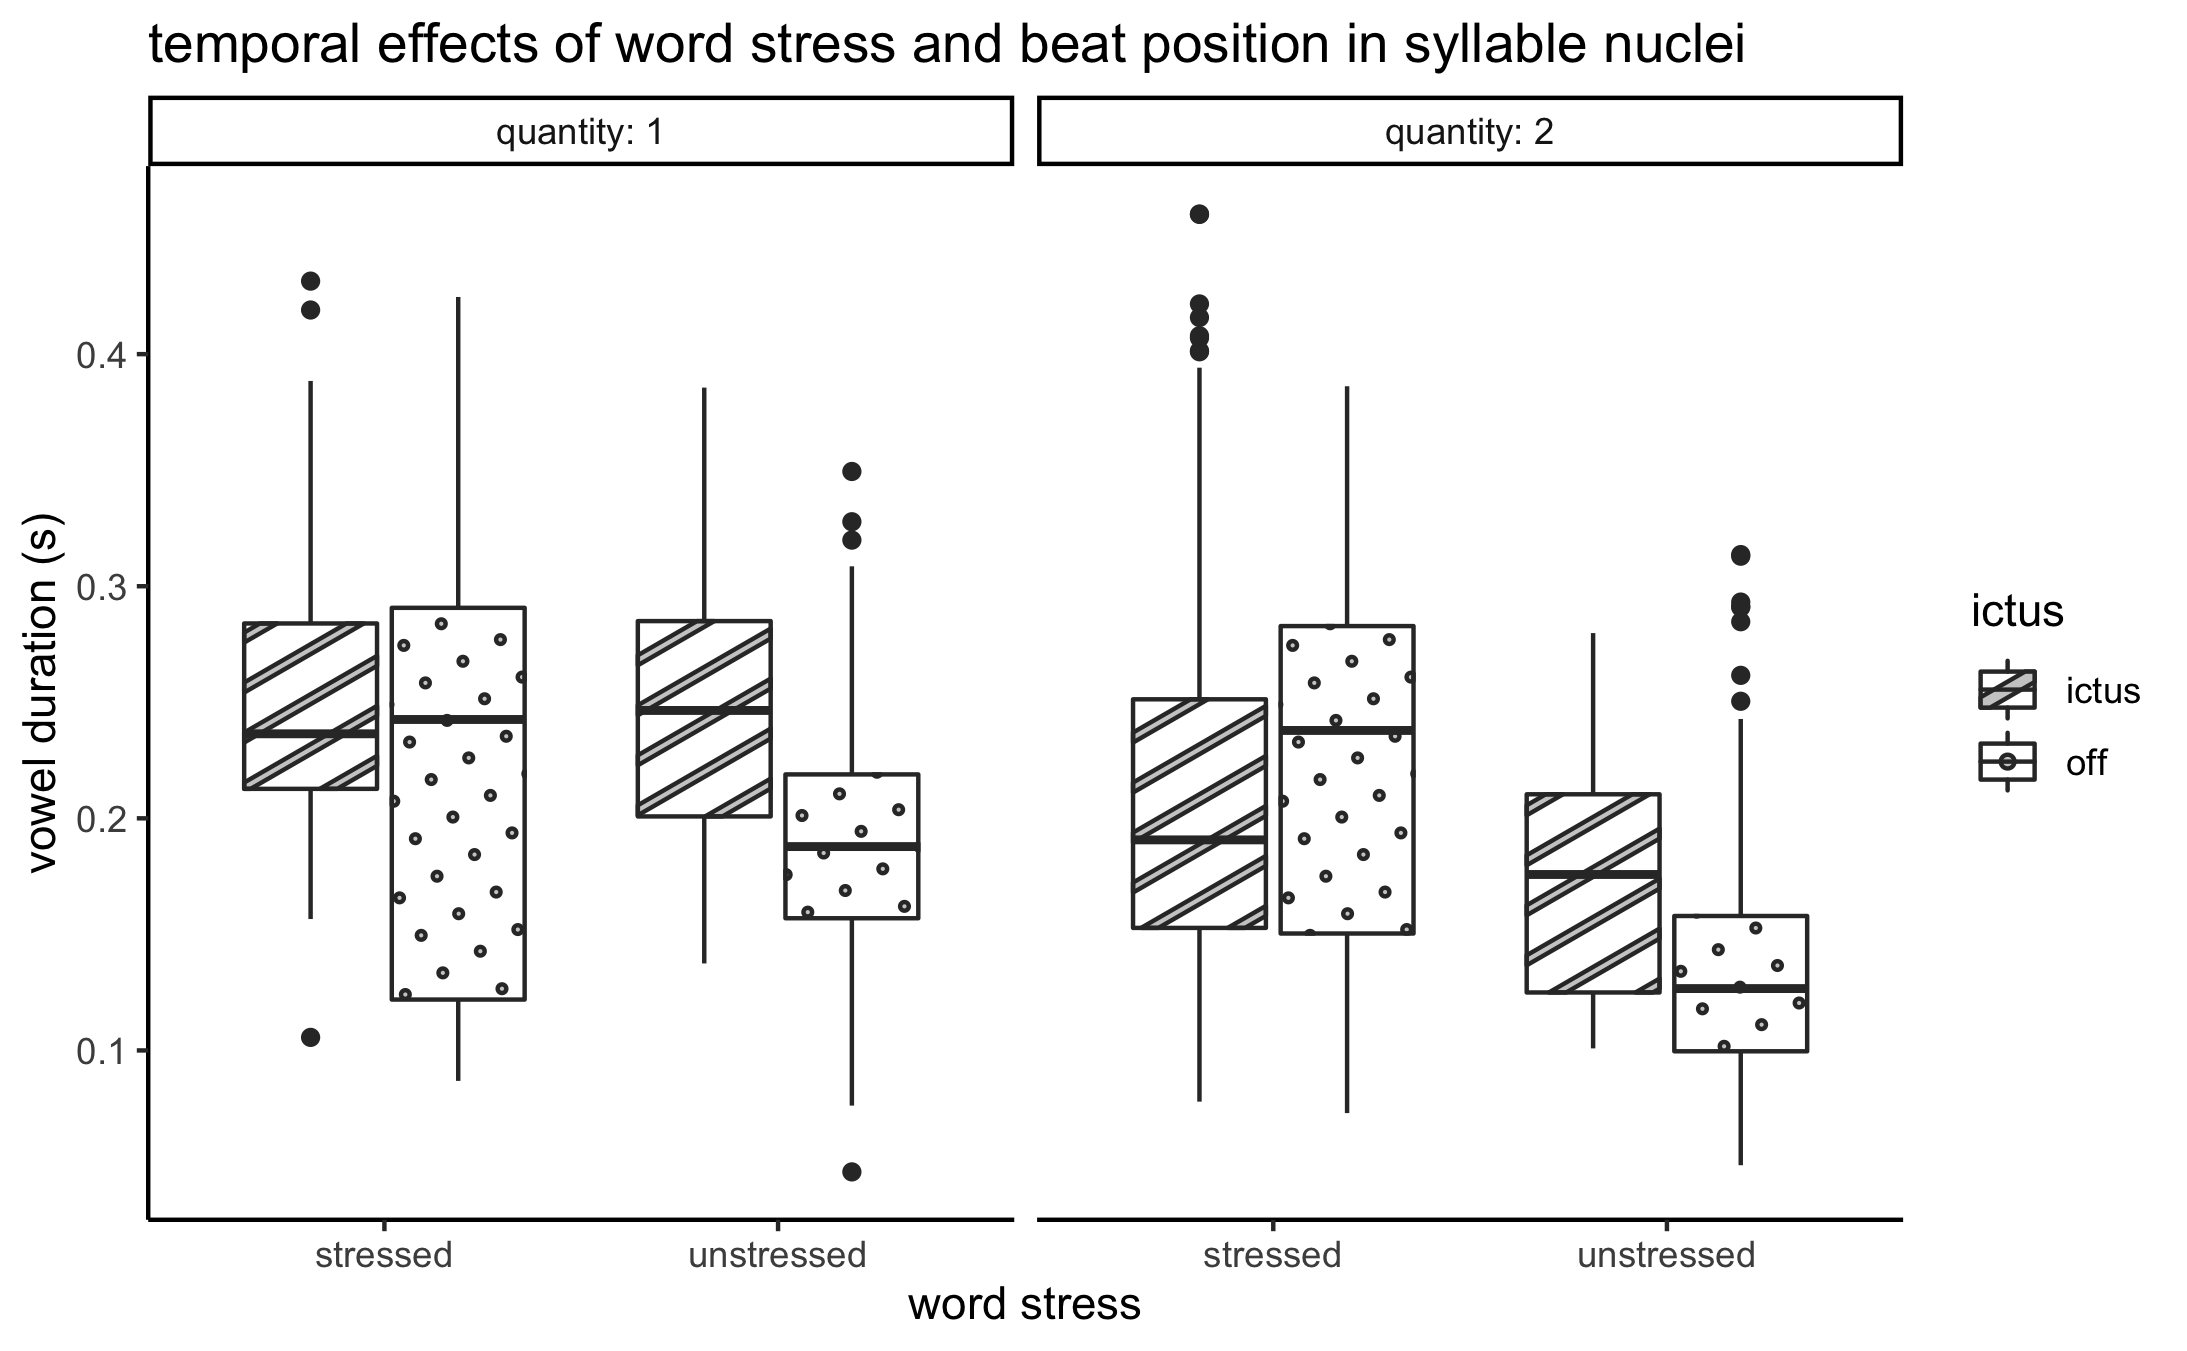
\includegraphics[width = \textwidth]{/Users/sarah/Git/regilaul_project/manuscript/results/dur_density_qfac.png}
\caption{vowel durations of stressed and unstressed Q1 and Q2 syllables falling on (ictus) and off the beat}
\label{durstrick}
\end{figure}

The two graphs in \ref{durstrick} illustrate the distribution of vowel durations in stressed and unstressed syllables falling on and off the beat. In Q1 syllables, ictus position predicts longer vowels in both stressed and unstressed syllables, while stressed syllables are longer overall than unstressed. In Q2, we see longer vowel durations for ictus position in stressed syllables, and higher means for ictus position in unstressed, though the distributions overlap much more here. \\

Linear mixed-effects model results are significant for off-ictus (p<0.05**), stressed (p<0.001***), and Q2 (p<0.001***). 

\begin{figure}[htpb]
\centering
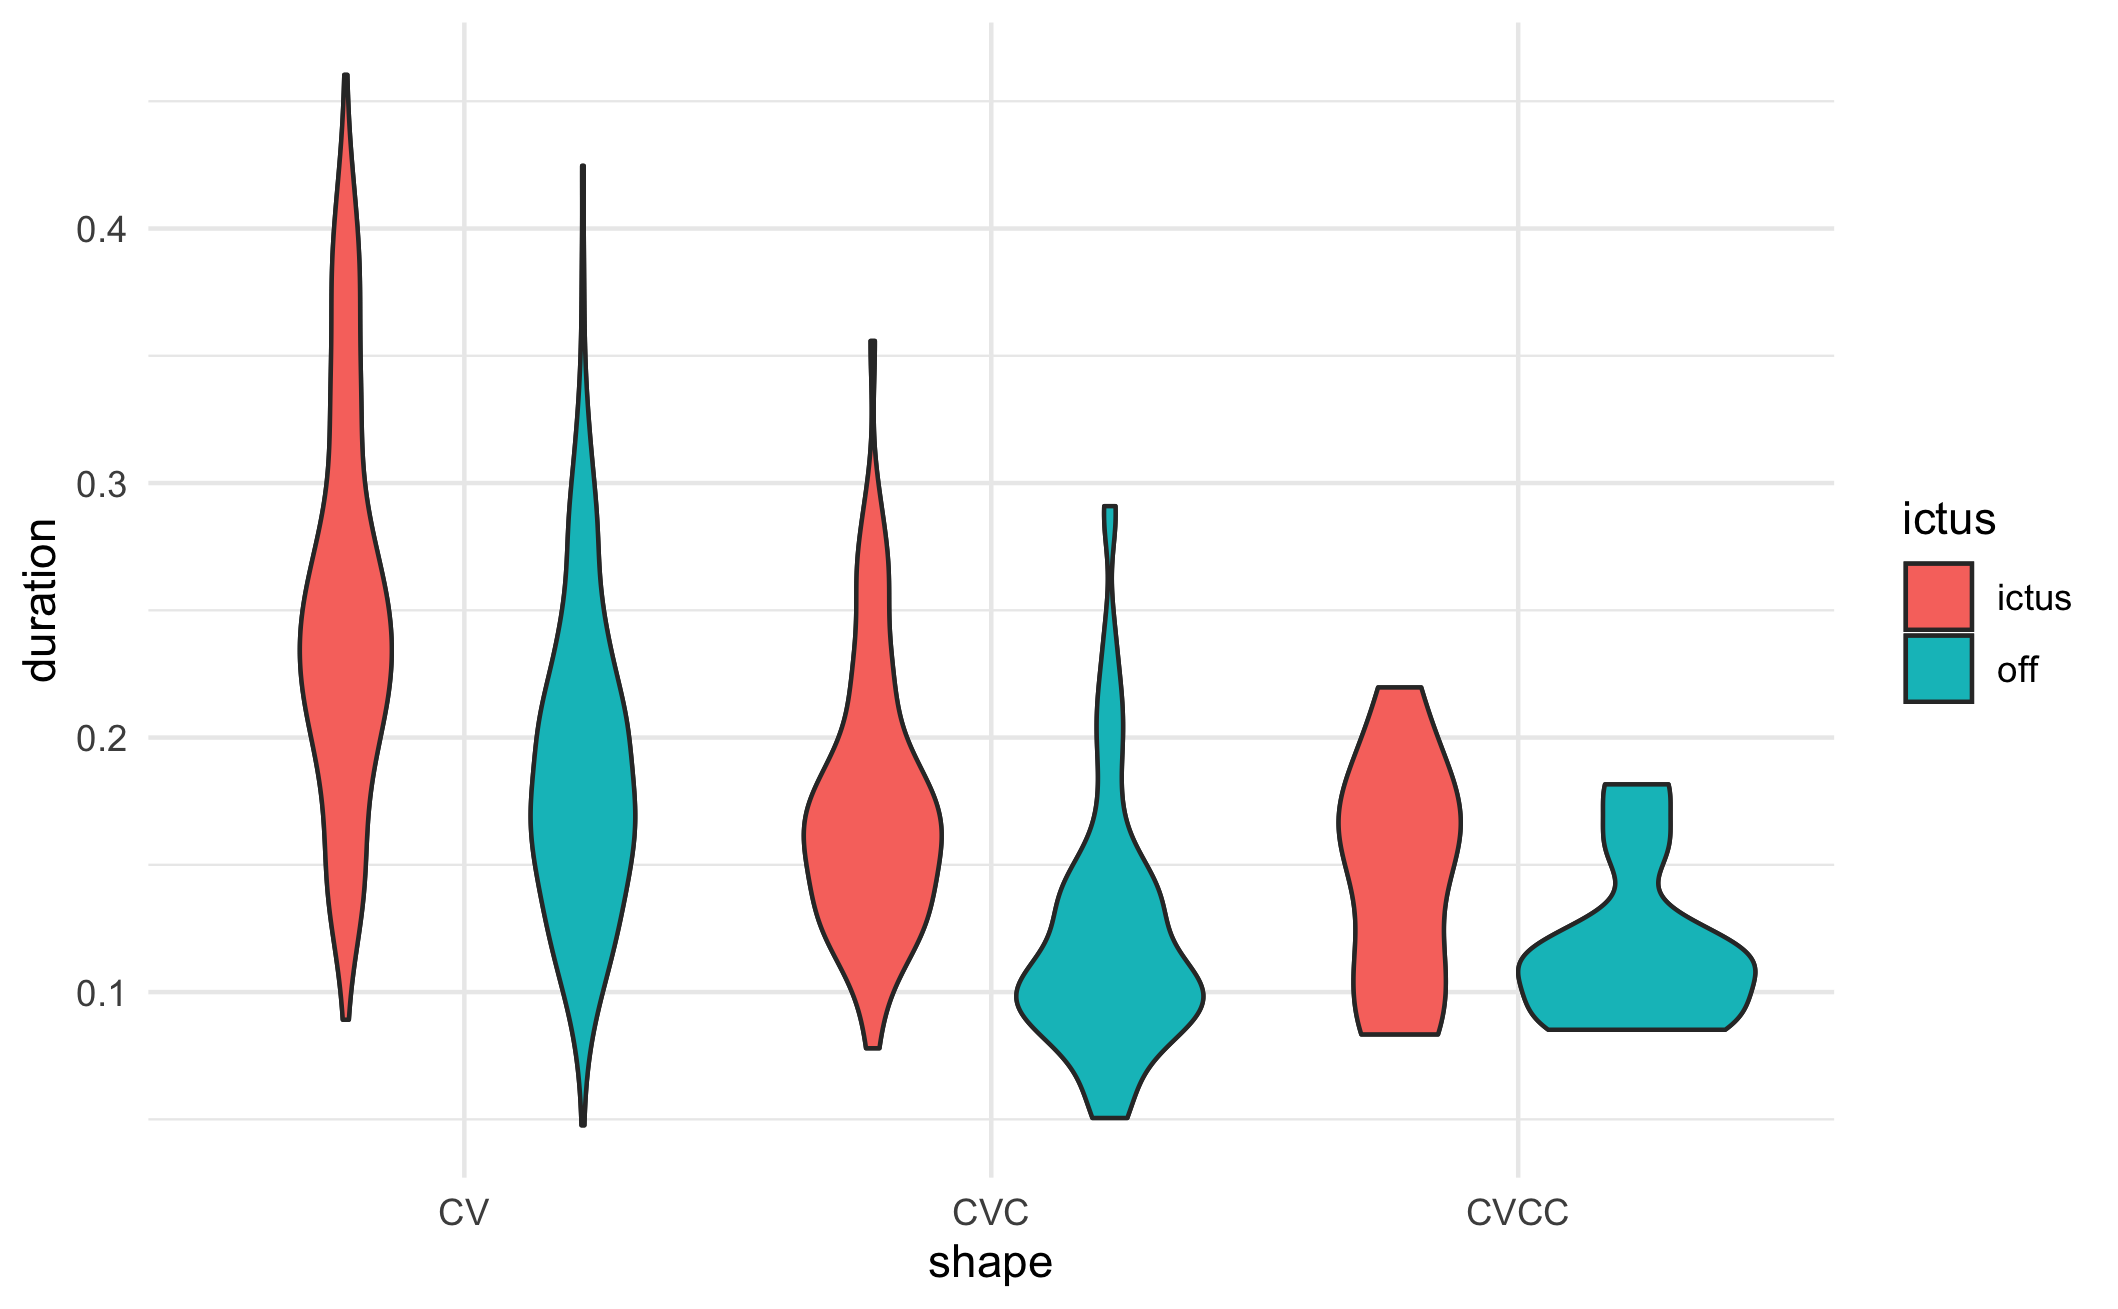
\includegraphics[width=\textwidth]{/Users/sarah/Git/regilaul_project/manuscript/results/dur_shape_ictus.png}
\caption{vowel dur(s) by beat position and syll. shape}
\label{ickdursh}
\end{figure}

Compared to Q1 unstressed syllables in ictus position (the intercept,  off-ictus positions have a negative slope and are overall shorter. Stressed syllables have a small positive slope, indicating longer vowel durations. Q2 syllables have a negative slope, highlighting the shortening of syllable nuclei to accomodate the codas of these syllables. 


\begin{figure}[htbp]
\centering
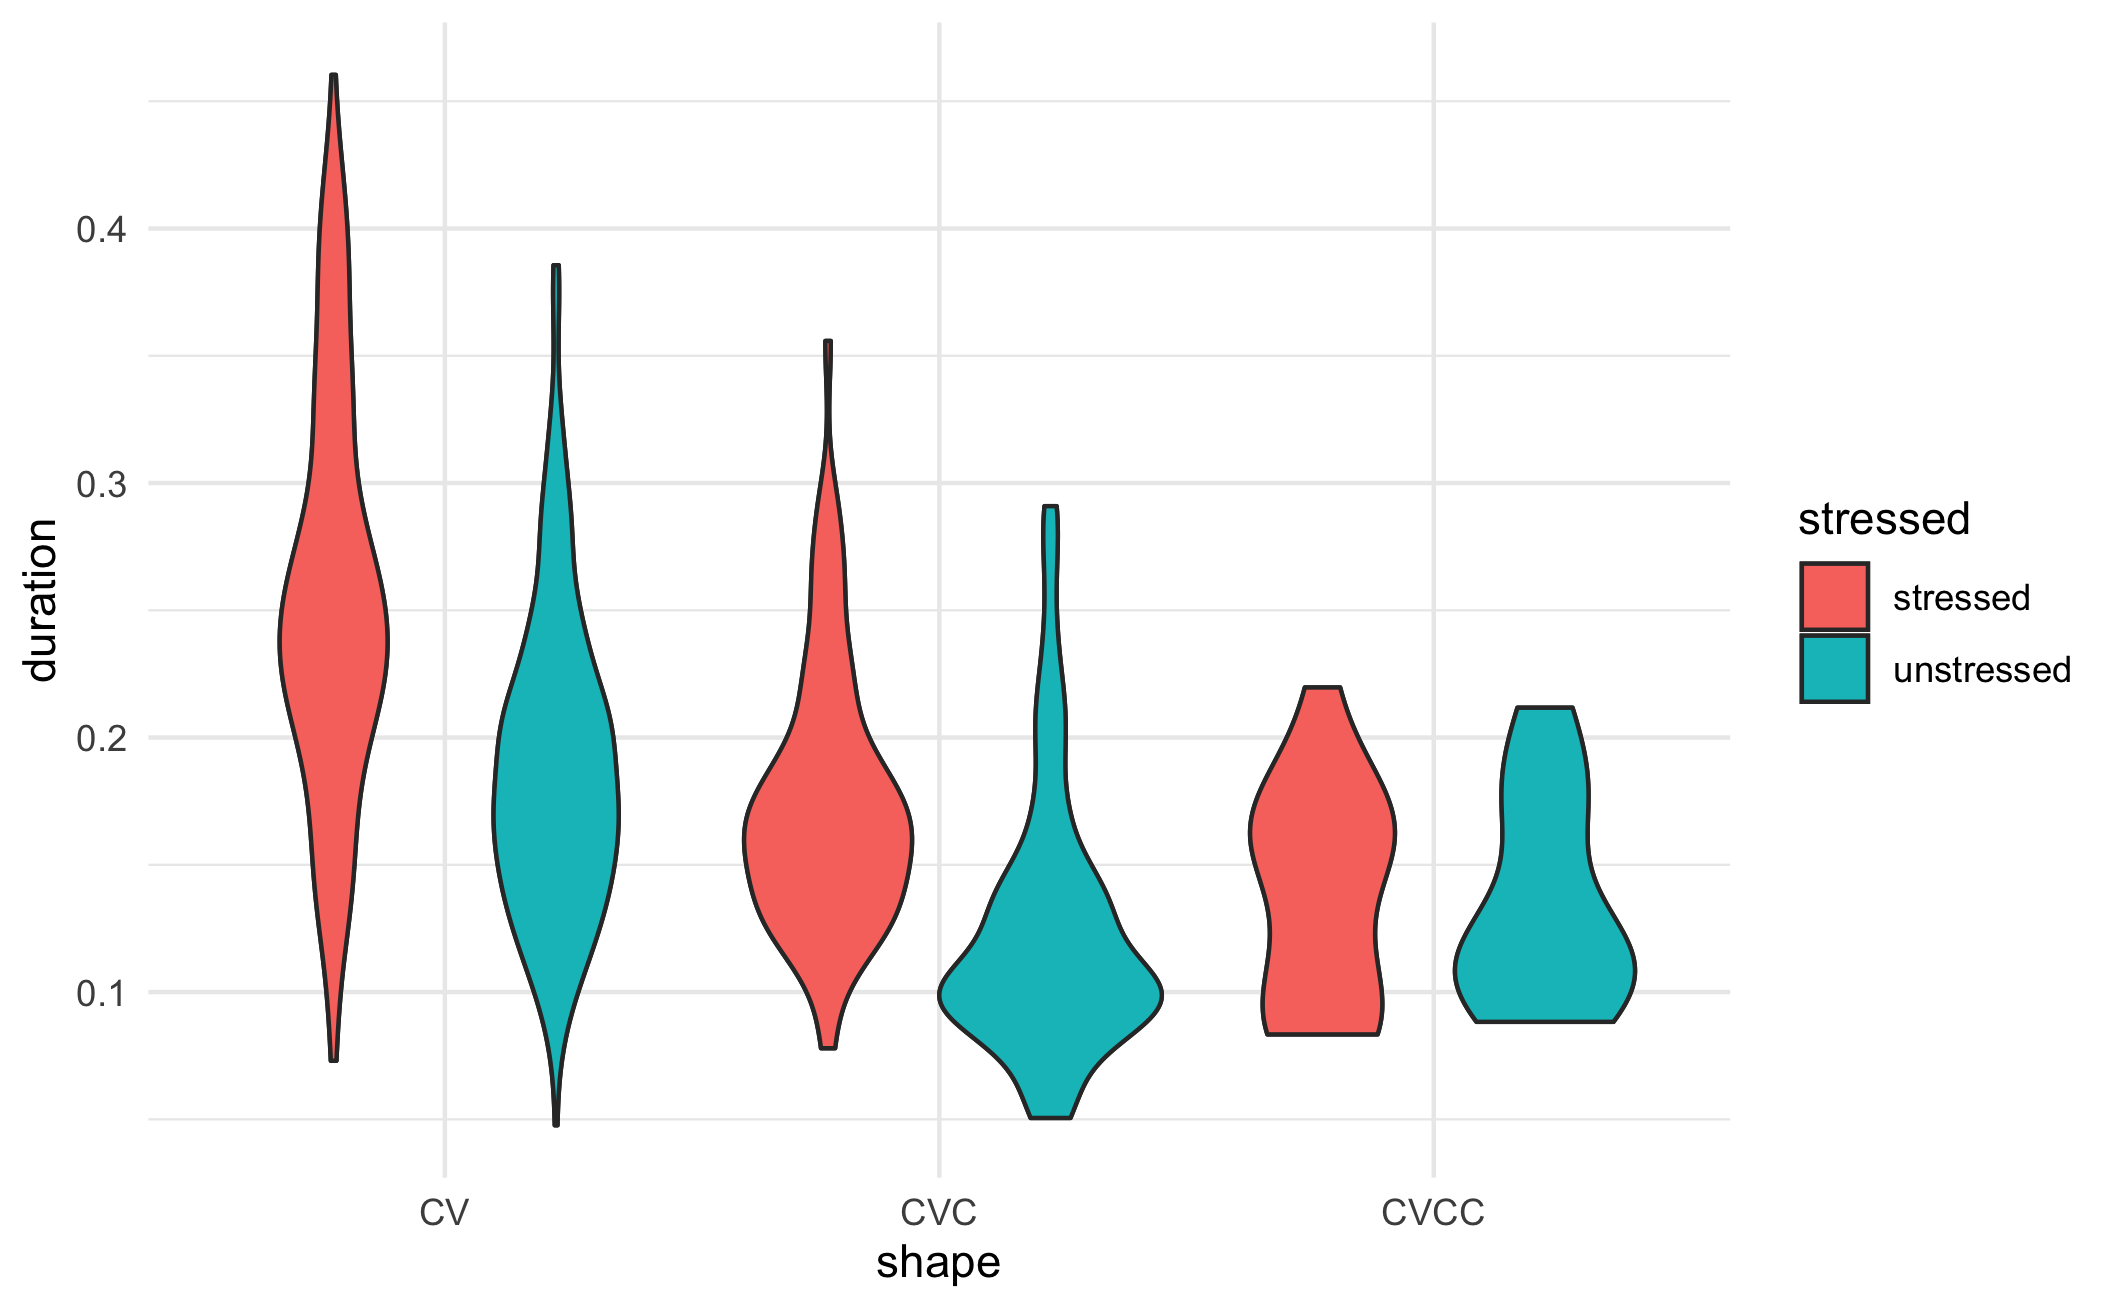
\includegraphics[width=\textwidth]{/Users/sarah/Git/regilaul_project/manuscript/results/dur_shapestress.png}
\caption{vowel dur(s) by word stress and syll. shape}
\label{strdursh}

\end{figure}
Anova comparison of the maximal design model with a null model is also statistically significant (p<0.001***). I reject the null hypothesis: these results support both word-level stress and beat position in song (ictus) as predictors for vowel duration. 

The graph in \ref{ickdursh} illustrates the distribution of vowel durations in different syllable shapes falling on and off the beat. 

A similar pattern can be seen in \ref{strdursh}, where the stressed or unstressed status is shown instead. At both song and word levels of prominence, CV or Q1 syllables are the longest, gradually decreasing in CVC and CVCC, both of which are Q2 syllables.  This further confirms the gradience of the quantity contrast at the segmental level. 



%%%%%%%%%%%%%%%%%%%%%%%%%%%%%%%%%%%%%%%%%%

%
%%%%%%%%%%%%

\subsection{Vowel Dispersion}
A subset of the Q1 and Q2 vowels used for duration measurements above is taken,  containing only those five vowel phonemes which occur in both stressed and unstressed syllables at the word level: \[a, e, i, o, u\]. The total number of vowels in this set is {\bf N}.
To account for physiological differences between singers, vowel dispersion is calculated as the euclidean distance of each token from the respective singer's vowel center in the (F1, F2) space. 


\begin{figure}[htbp]
\centering
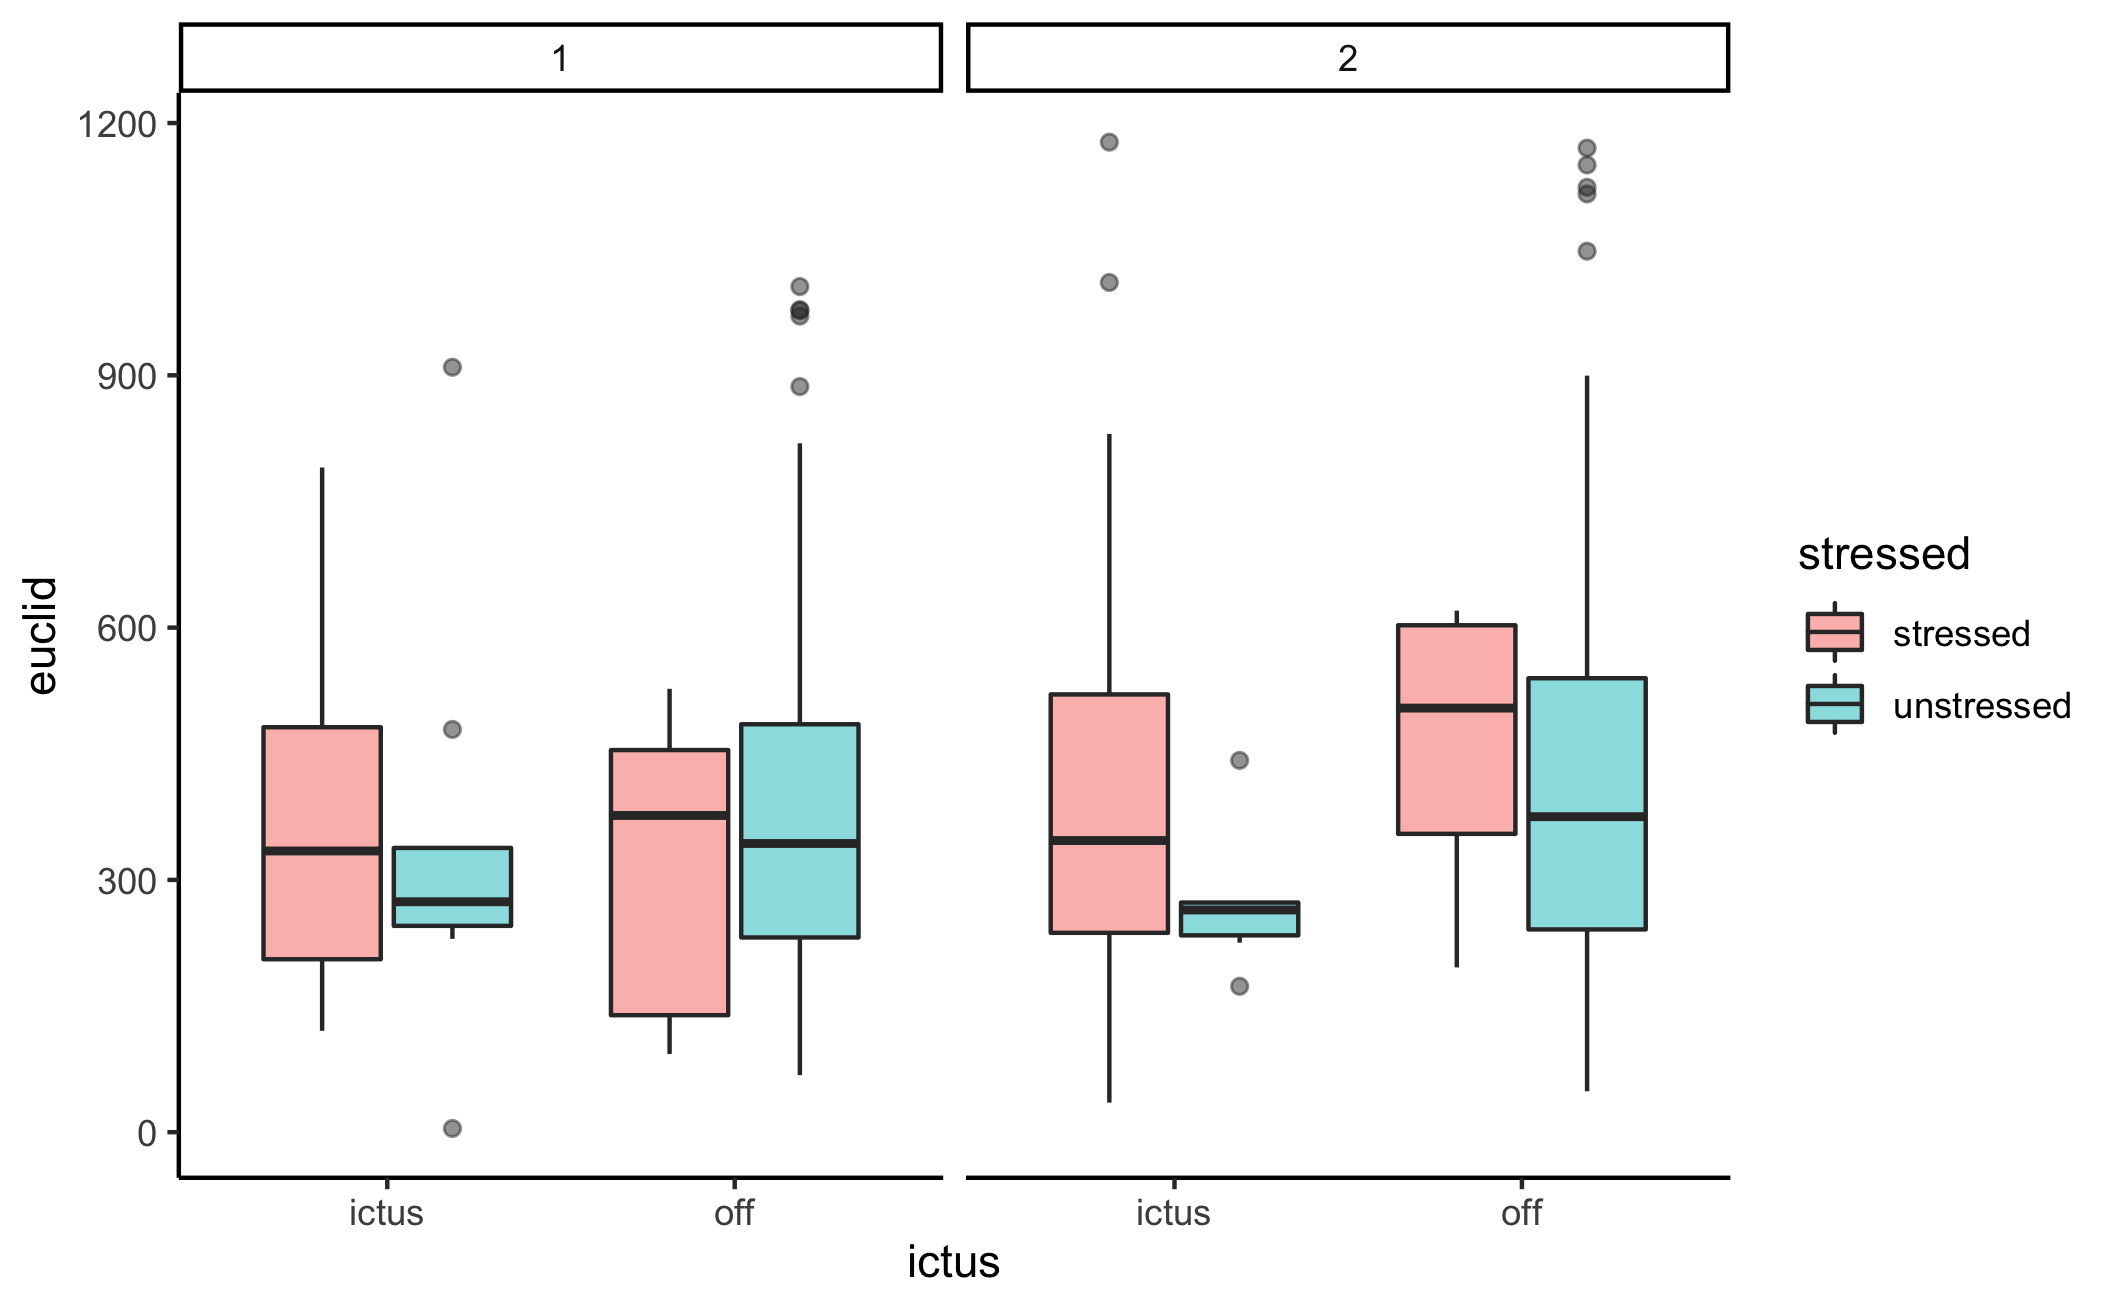
\includegraphics[width=\textwidth]{/Users/sarah/Git/regilaul_project/manuscript/results/space_strictus.png}
\caption{euclidean distance of vowels in stress and ictus}
\label{spcstrick}

\end{figure}
A pattern is marginally visible in the two graphs  \ref{spcstrick}, faceted by Q1 and Q2. Notice that in off-ictus position, vowel dispersion means of stressed syllables are higher than those of stressed syllables in ictus position. This indicates that stressed syllables falling off the beat are being compensated for their shortened vowels by way of increased articulation of quality. This pattern, however, doesn't shake out as statistically significant in the model. \\
A linear mixed effects model for vowel dispersion is constructed, but only the uninterpretable intercept shows significance. 
Comparison with null model is not statistically significant. Thus in the case of vowel dispersion, we fail to reject the null hypothesis. This could be due to the relatively smaller size of the data subset. 



\chapter{Discussion}
\index{Discussion@\emph{Discussion}}%

\section{Temporal Prosodic Features Crystalized at Segmental level in isochronous syllables}

These results support the hypothesis that prosodic timing modifications resulting from the synchronization of independent rhythms (in this case, syllables and notes into syllable-notes) do not result in the subordination of one system to another. In this case, when syllables and notes become one timing unit, the temporal acoustic correlates often found at suprasegmental levels (syllable, foot, word) are found at the segmental levels. 

This interaction is then more analagous to entrainment of two independent rhythmic systems than to language being forcibly pigeon-holed into the metrical structure of music. 


%\section{Vowel Dispersion}
%Results for the predictive power of ictus and off-ictus, stressed and unstressed syllables and vowel space dispersion were not significant. The patterns that seem to emerge visually in the graphs of distributions suggest that the situation might be ameliorated by increasing the dataset. For this measurement, there were fewer available tokens than for vowel duration, and therefore less statistical power. Further examination is needed to determine whether or not the observed pattern is simply lacking in power or whether the premises that lead to this hypothesis are missing something entirely. 


\section{Future Studies} 

This study used a sample of nine songs and three singers, all recorded in the 1960s. Annotation has already begun on the remaining songs that fit into this sample's criteria: In total, there are seventeen songs and seven singers from Parnumaa county recorded in the 1960s.
% Increasing the size of the audio corpus would facilitate exploratory analysis in countless dimensions of music and language, and also shed light on the issue of vowel space unresolved here. 
Several of the singers featured in this sample set were also recorded speaking. Annotating their natural speech would provide a valuable contribution to the song corpus, as findings from the songs could be compared with speech of the same person.  

Extending the findings of vowel duration and the ternary quantity contrast has several obvious paths: synchronic analysis of with song samples from the same approximate time period but differing according to region, or even language: several other Balto-Finnic families have a trochaic tetrameter folksong tradition. Diachronic analysis with song samples of same singers in the same region at different points in time is another possibility with data from the Estonian Folklore Archives. Both these goals are achievable only with the continued annotation of the corpus of regilaul, which is quite demanding work. As I continue to build this corpus, I am also actively exploring ways in which to automate the process. The inclusion of beat tracking software eliminated much observer subjectivity, and also facilitated the forced-aligner: by automatically grouping verse lines into measures, the aligner was given phrase groupings to synthesize and compare, rather than attempting to align the entire song in a linear fashion. However, as the forced aligner used here was made specifically for speech, one way to improve the accuracy of the forced aligner (decreasing manual adjustment of annotations) would be to train a the aligner on sung material using supervised machine learning. As I plan to continue with the annotations either way, I can use the corrections I make as training material for the algorithm, with the hopeful result that the forced-aligner will eventually reach some threshold of accuracy, voiding the need for manual adjustments. 

\section{ML plans outline}
%Kaldi: uses DNN (Deep Neural Net) rather than linear model like MFA (montreal forced-aligner). 

%https://www.kaldi-asr.org/doc/
%https://www.eleanorchodroff.com/tutorial/kaldi/index.html

for several/general uralic languages \citep{leinonen2021}. 
Would be good to try for other runosongs! 

%https://github.com/lingsoft/aalto-kaldi-align-elg

for Estonian specifically \citep{ratsep2022}
\section{Conclusion}

This study examined fine-grained acoustic-phonetic features of Estonian prosody in the context of traditional folksongs known as regilaul. The data support the hypothesis that duration contrasts inherent in the ternary quantities of Estonian are still present at the segmental level, even after undergoing modification to fit syllables into isochronous notes of the song. The data also supports that the durational correlates of word-level stress are also crystallized and evident at the segmental level, so while it isn't lexically contrastive, the role of primary stress and unstress to mark word boundaries in spoken Estonian is still present in sung Estonian. 
%Vowel quality patterns were measured but not significant for this dataset. 

This indicates a relationship more akin to the collaboration of two independent rhythmic systems rather than one rhythmic system dominating the other. Combined with the fact that any regilaul text can be sung to any existing regilaul melody brings into question whether {\it spoken} metrical verse text is truly independent of the temporal constraints of the musical meter they are made with, or somewhere between language and music. 




%%%%%%%%%%%%%%%%%%%%%%%%%%%%%%%%%%%%%%%%%%%%%%%%%%%%%%%%%%%%%%%%%%%%%%
% Appendix/Appendices                                                %
%%%%%%%%%%%%%%%%%%%%%%%%%%%%%%%%%%%%%%%%%%%%%%%%%%%%%%%%%%%%%%%%%%%%%%
%
% If you have only one appendix, use the command \appendix instead
% of \appendices.
%%
\appendices
\index{Appendices@\emph{Appendices}}%
%
\chapter{lmer output}
\footnote{Signif. codes:   ‘***’ 0.001 ‘**’ 0.01 ‘*’ 0.05 }
\begin{table}[htbp]
\caption{duration \& syllable quantity}
\begin{center}
\begin{tabular}{|l|c|c|c|}
\hline
{\bf Predictors}	&	{\bf Estimates}	&	{\bf Confidence Interval}	&	{\bf p}	\\
\hline
\hline
(Intercept)	&	0.27	&	0.23 – 0.30	&	<0.001***	\\
Q2	&	-0.04	&	-0.06 – -0.02	&	<0.001***	\\
Q3	&	-0.03	&	-0.06 – -0.00	&	0.048*	\\
off-ictus &	-0.05	&	-0.08 – -0.02	&	0.004*	\\
Q2 * off-ictus	&	0.02	&	-0.03 – 0.06	&	0.54	\\

Q3 *off-ictus	&	-0.02	&	-0.07 – 0.03	&	0.44	\\
\hline
\hline
$\sigma^2$ 	&	0.0012	&		&		\\
$\tau_{00}$ word	&	0.0034	&		&		\\
$\tau_{00}$ song	&	0.0022	&		&		\\
$\tau_{00}$ performer	&	0.0001	&		&		\\
ICC	&	0.8227	&		&		\\
\hline
\hline
N song	&	9	&		&		\\
N word	&	298	&		&		\\
N performer	&	3	&		&		\\
Observations	&	367	&		&		\\
Marginal R2 / Conditional R2	&	0.071 / 0.835	&		&		\\
\hline
\end{tabular}
\end{center}
\label{qdurrandoms}
\end{table}%



%%%%%%%%%%


\begin{table}[htb]
\caption{duration \& syllable quantity: model comparison (max to null)}
\centering
\begin{tabular}{|ccccccccc|}
\hline
      & npar   &  AIC   &  BIC & logLik & deviance  & Chisq & Df & Pr(>Chisq)    \\
      \hline
      \hline
null  &  5 &-914.74 &-895.21 &462.37  &-924.74        &&& \\                 
design  &  10 &-949.20 &-910.15 &484.60 & -969.20 & 44.464  &5  &1.865e-08 *** \\
\hline

\end{tabular}
\label{qcomp}
\end{table}%
%%%%%%%


\begin{table}[htb]
\caption{duration \& stress and ictus: model comparison (max to null) }
\begin{center}
\centering
\begin{tabular}{|ccccccccc|}
\hline
      & npar   &  AIC   &  BIC & logLik & deviance  & Chisq & Df & Pr(>Chisq)    \\
\hline
\hline
null &   5& -1747.0 &-1724.4  &878.5 & -1757.0         && \\            
design &   10& -1966.8& -1921.6  &993.4  &-1986.8 & 229.81&  5 & < 2.2e-16 ***\\
\hline

\end{tabular}
\end{center}
\label{durstrickmdls}
\end{table}%

%
%\begin{equation*}
%
%des_null_md: euclid ~ (1 | segment) + (1 | song) + (1 | performer) \\
%desmd: euclid ~ stressed + ictus + stressed * ictus + (1 | segment) + (1 | song) + (1 | performer) \\
%\end{equation*}





\begin{table}[htb]
\caption{duration \& stress-ictus}
\begin{center}
\begin{tabular}{|l|c|c|c|}
\hline
\hline
Predictors	&	Estimates	&	Confidence Intervals	&	p	\\
\hline
(Intercept)	&	0.22	&	0.18 – 0.25	&	<0.001***	\\
off-ictus	&	-0.03	&	-0.05 – -0.00	&	0.017**	\\
stressed	&	0.05	&	0.03 – 0.07	&	<0.001***	\\
Q2&	-0.05	&	-0.06 – -0.04	&	<0.001***	\\
off-ictus* stressed	&	-0.01	&	-0.04 – 0.02	&	0.467	\\
off-ictus* Q2	&	0.01	&	-0.01 – 0.03	&	0.332	\\
\hline
\hline
$\sigma^2$ 	&	0.0026	&&	\\
$\tau_{00}$ word	&	0.0004	&&	\\
$\tau_{00}$ song	&	0.0018		&&	\\
$\tau_{00}$ performer	&	0.0001		&&\\
ICC	&	0.4761	&&	\\
\hline
\hline
N word	&	315		&&	\\
N song	&	9		&&	\\
N performer	&	3	&&	\\
Observations	&	676	&&	\\
Marginal R2 / Conditional R2	&	0.190 / 0.576	&&\\
\hline
\end{tabular}
\end{center}
\label{durlmerrando}
\end{table}%

%%%space
%%%%%%%%%%%

\begin{table}[htb]
\caption{euclidean distance dependent fixed effects}
\begin{center}
\begin{tabular}{|l|c|c|c|}
\hline							
Predictors	&	Estimates	&	Confidence Interval	&	p	\\
\hline
\hline
(Intercept)	&	351.9	&	207.53 – 496.26	&	<0.001***	\\
stressed 	&	48.7	&	-48.46 – 145.87	&	0.325	\\
off-ictus	&	80.8	&	-14.93 – 176.52	&	0.098	\\
stressed*off-ictus	&		&		&		\\
\hline							
\hline
$\sigma^2$	&	32259.12			&&		\\
$\tau_{00}$ segment	&	4058.78		&&			\\
$\tau_{00}$  song	&	5512.35				&&	\\
$\tau_{00}$  performer	&	5432.4				&&	\\
ICC	&	0.32		&&			\\
\hline
\hline
N segment	&	11		&&			\\
N song	&	9				&&	\\
N performer	&	3		&&			\\
Observations	&	401				&&	\\
Marginal R2 / Conditional R2	&	0.008 / 0.323		&&			\\									
\hline							
\end{tabular}
\end{center}
\label{randolmereuc}
\end{table}%


\begin{table}[htb]
\caption{euclidean distance \& stress-ictus: model comparison (max to null) }
\begin{center}
\centering
\begin{tabular}{|ccccccccc|}

\hline
     &       npar  &  AIC   & BIC  & logLik & deviance  & Chisq & Df & Pr(>Chisq) \\
     \hline
     \hline
null  &  5 & 5347.3 & 5367.3 & -2668.7  & 5337.3             \\        
design    &      8 & 5348.7& 5380.7 &-2666.4  & 5332.7 & 4.5855 & 3   &  0.2048 \\
\hline
\end{tabular}
\end{center}
\label{aoveuc}
\end{table}%


%\begin{figure}[htb]
%\centering
%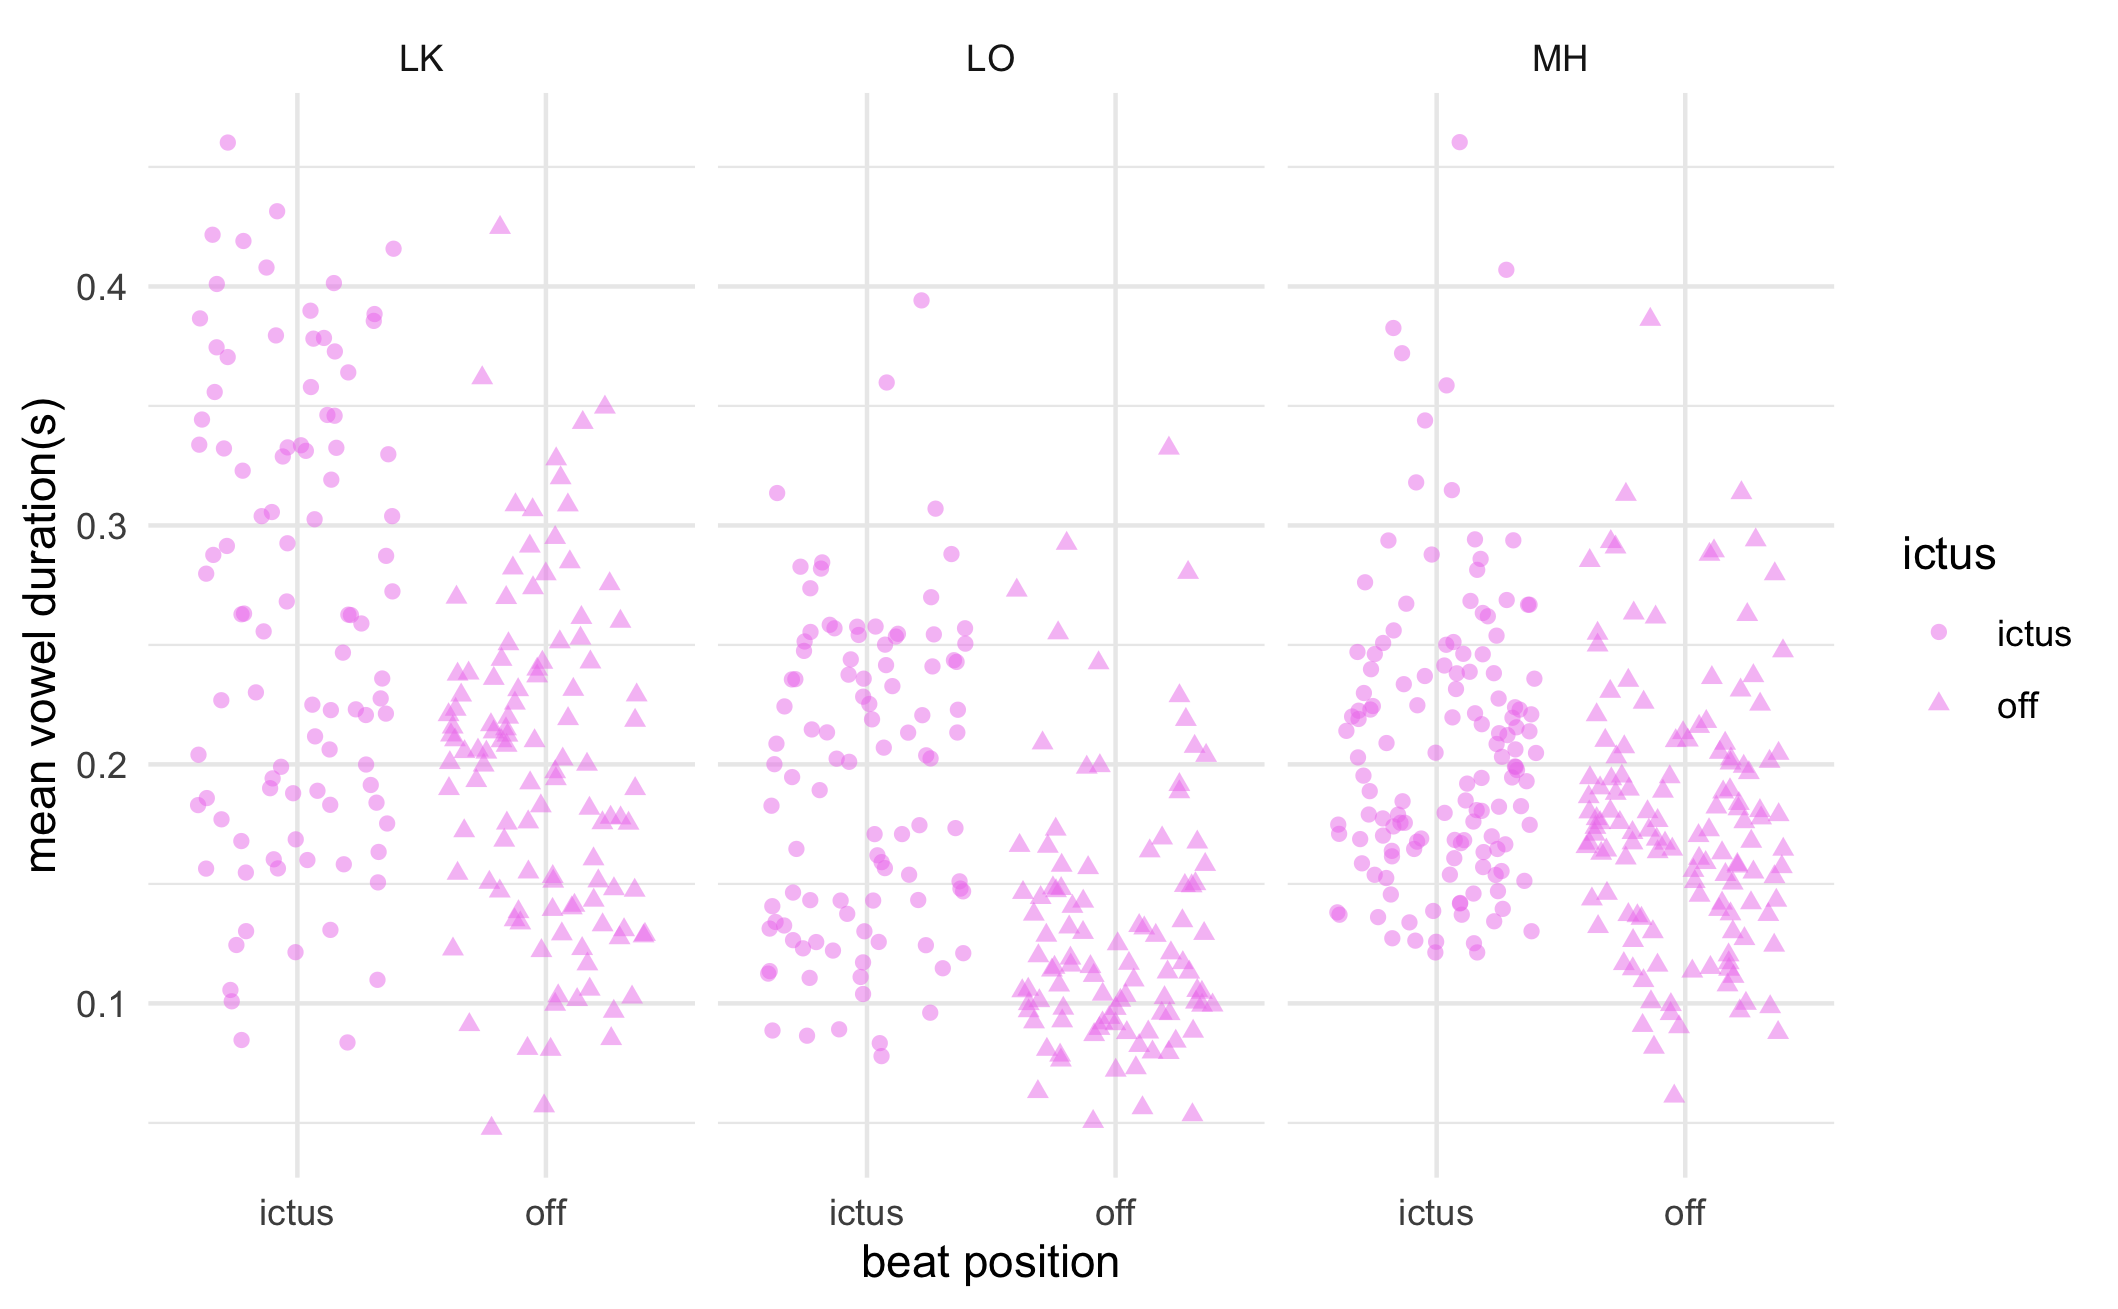
\includegraphics[width=\textwidth]{/Users/sarah/Git/regilaul_project/manuscript/results/perf_ick_dur.png}
%
%\caption{vowel durations on and off the beat in each performer}
%\label{perfbeats}
%
%
%\end{figure}



%

%
%%%%%%%%%%%%%%%%%%%%%%%%%%%%%%%%%%%%%%%%%%%
\chapter{My Appendix \#3}
\index{Appendix!My Appendix \#3@\emph{My Appendix \#3}}%

\section{The First Section}
This is the first section.
This is the third appendix.

\section{The Second Section}
This is the second section of the third appendix.





%%%%%%%%%%%%%%%%%%%%%%%%%%%%%%%%%%%%%%%%%%%%%%%%%%%%%%%%%%%%%%%%%%%%%%
% Generate the bibliography.					     %
%%%%%%%%%%%%%%%%%%%%%%%%%%%%%%%%%%%%%%%%%%%%%%%%%%%%%%%%%%%%%%%%%%%%%%
%								     %
% NOTE: For master's theses and reports, NOTHING is permitted to     %
%	come between the bibliography and the vita. The command      %
%	to generate the index (if used) MUST be moved to before      %
%	this section.	
\printindex%    % Include the index here. Comment out this line      %
%		% with a percent sign if you do not want an index.   %					     %
%								     %
%\nocite{*}      % This command causes all items in the 		     %
                % bibliographic database to be added to 	     %
                % the bibliography, even if they are not 	     %
                % explicitly cited in the text. 		     %
		%						     %
\bibliographystyle{apa-good.bst}  % Here the bibliography 		     %
\bibliography{regilaul}        % is inserted.			     %
\index{Bibliography@\emph{Bibliography}}%			     %
%%%%%%%%%%%%%%%%%%%%%%%%%%%%%%%%%%%%%%%%%%%%%%%%%%%%%%%%%%%%%%%%%%%%%%


%%%%%%%%%%%%%%%%%%%%%%%%%%%%%%%%%%%%%%%%%%%%%%%%%%%%%%%%%%%%%%%%%%%%%%
% Generate the index.						     %
%%%%%%%%%%%%%%%%%%%%%%%%%%%%%%%%%%%%%%%%%%%%%%%%%%%%%%%%%%%%%%%%%%%%%%
%								     %
% NOTE: For master's theses and reports, NOTHING is permitted to     %
%	come between the bibliography and the vita. This section     %
%	to generate the index (if used) MUST be moved to before      %
%	the bibliography section.				     %
%								     %

%%%%%%%%%%%%%%%%%%%%%%%%%%%%%%%%%%%%%%%%%%%%%%%%%%%%%%%%%%%%%%%%%%%%%%


%%%%%%%%%%%%%%%%%%%%%%%%%%%%%%%%%%%%%%%%%%%%%%%%%%%%%%%%%%%%%%%%%%%%%%
% Vita page.							     %
%%%%%%%%%%%%%%%%%%%%%%%%%%%%%%%%%%%%%%%%%%%%%%%%%%%%%%%%%%%%%%%%%%%%%%

%\begin{vita}
%Sarah Marie Ransom-Laud
%was born in Sarasota, Florida on 11 July 1990. Her early career was as a songwriter and recording artist, releasing several full-length albums combining digital and analog recording methods over the last decade. 
%
%In 2018 she received the Bachelor of Arts degree in Linguistics from the University of Wisconsin, Milwaukee. Upon graduation, she moved to Austin with her partner, Kavi, and taught English as a Second Language (ESL) to adults until her admission into the PhD program in the department of Linguistics at the University of Texas at Austin, where she matriculated in Fall 2019. 


%\end{vita}

\end{document}
